\documentclass{elsart}
%\documentclass[journal,twoside]{IEEEtran}
%\usepackage{natbib}
\usepackage{array}
\usepackage{color}
\usepackage{cite}
\usepackage{url}
\usepackage{epsfig}
\usepackage{psfrag}
\usepackage{pstricks}
\usepackage{acronym}
\usepackage{subfigure}
\usepackage{units}
\usepackage{amsmath}
\usepackage{units}
\usepackage{vmargin}
\setpapersize{USletter}
\setmarginsrb{1in}{1in}{1in}{1in}{0pt}{0mm}{36pt}{36pt}


\usepackage{acronym}
% ACRONYMS
\acrodef{ADT}{Abstract Data Type}
\acrodef{API}{Application Program Interface}
\acrodef{APNG}{Animated Portable Network Graphics}
\acrodef{AVIRIS}{Airborne Visible InfraRed Imaging Spectrometer}
\acrodef{bil}{Band Interleave by Line}
\acrodef{bip}{Band Interleave by Pixel}
\acrodef{bsq}{Band Sequential}
\acrodef{CaSIL}{California Spatial Information Library}
\acrodef{CEO:P}{Cyberinfrastructure for Environmental Observatories: Prototype Systems to Address Cross-Cutting Needs}
\acrodef{CERES}{California Environmental Resources Evaluation System}
\acrodef{CIMIS}{California Irrigation Management Information System}
\acrodef{COMET}{\emph{Coast-to-Mountain Environmental Transect}}
\acrodef{CPU}{Central Processing Unit}
\acrodef{CQ}{Continuous Query}
\acrodef{CRA}{California Resources Agency}
\acrodef{CRS}{Coordinate Reference System}
\acrodef{CSDGM}{Content Standard for Digital Geospatial Metadata}
\acrodef{DAAC}{Distributed Active Archive Center}
\acrodef{DAG}{Directed Acyclic Graph}
\acrodef{dbms}[D\textsc{bms}]{database management system}
\acrodef{DCT}[DCT]{Dynamic Cascade Tree}
\acrodef{DFS}{Depth First Search}
\acrodef{DNF}{Disjunctive Normalized Form}
\acrodef{DWR}{Department of Water Resources}
\acrodef{dsms}[D\textsc{sms}]{data stream management system}
\acrodef{EPA}{Environmental Protection Agency}
\acrodef{EOS}{Earth Observing System}
\acrodef{EPSG}{European Petroleum Survey Group}
\acrodef{ERTS}{Earth Resources Technology Satellite}
\acrodef{ESRI}{Environmental Systems Research Institute}
\acrodef{GIS}{Geographic Information Systems}
\acrodef{GLT}{Geographic Lookup Table}
\acrodef{GML}{Geography Markup Language}
\acrodef{GMLJP2}{GML in JPEG 2000}
\acrodef{GOES}{Geostationary Operational Environmental Satellite}
\acrodef{GPS}{Global Positioning System}
\acrodef{GRASS}{Geographic Resources Analysis Support System}
\acrodef{GS}[\emph{GeoStreams}]{GeoStreams}
\acrodef{GUI}{Graphical User Interface}
\acrodef{GVAR}{G\textsc{oes} VARiable}
\acrodef{HTML}{HyperText Markup Language}                           
\acrodef{IGFOV}{Instantaneous Geographic Field of View}
\acrodef{ISO}{International Standards Organization}
\acrodef{ITR}{Information Technology Research}
\acrodef{JPEG}{Joint Photographic Experts Group}
\acrodef{LACIE}{Large Area Crop Inventory Experiment}
\acrodef{LandSat}{Land Remote-Sensing Satellite}
\acrodef{LIDAR}{Light Detection and Ranging}
\acrodef{MDOP}{Multiple Data Ordering Page}
\acrodef{MNG}{Multiple-image Network Graphics}
\acrodef{MODIS}{Moderate Resolution Imaging Spectrometer} 
\acrodef{NASA}{National Aeronautics and Space Administration}
\acrodef{NCGIA}{National Center for Geographic Information and Analysis}
\acrodef{NDVI}{Normalized Difference Vegetation Index}
\acrodef{NEON}{National Ecological Observatory Network}
\acrodef{NOAA}{National Oceanic and Atmospheric Administration}
\acrodef{NPOESS}{National Polar-orbiting Operational Environmental Satellite System}
\acrodef{NRC}{National Research Council}
\acrodef{NSDI}{National Spatial Data Infrastructure}
\acrodef{NSF}{National Science Foundation}                      
\acrodef{OGC}{Open Geospatial Consortium}
\acrodef{OpenDAP}{Open-source Project for a Network Data Access Protocol}
\acrodef{OWS}{\ac{OGC} Web Services}
\acrodef{PIER}{Public Interest Energy Research}
\acrodef{PDL}{Perl Data Language}
\acrodef{PNG}{Portable Network Graphics}
\acrodef{QEG}{Query Execution Graph}
\acrodef{QEP}{Query Execution Plan}
\acrodef{QGIS}{Quantum GIS}
\acrodef{QM}{Query Manager}
\acrodef{RMSE}{Root Mean Squared Error}
\acrodef{ROI}{Region of Interest}
\acrodef{RPL}{Reverse Polish Lisp}
\acrodef{RSI}{Remotely-Sensed Imagery}
\acrodef{RSS}{Really Simple Syndication}
\acrodef{sdbms}[S\textsc{dbms}]{spatial database management system}
\acrodef{SIC}{Standard Industrial Classification}
\acrodef{SMS1}{Synchronous Meteorological Satellite 1}
\acrodef{STL}{Standard Template Library}
\acrodef{TIROS}{Television and Infrared Observation Satellite}
\acrodef{URL}{Uniform Resource Locator}
\acrodef{USGS}{U.S. Geological Survey}                           
\acrodef{UTM}{Universal Transverse Mercator}
\acrodef{XML}{eXtensible Markup Language}
\acrodef{WCS}{Web Coverage Service}
\acrodef{WKT}{Well Known Text}
\acrodef{WMS}{Web Map Services}
\acrodef{WRF}{Weather Research and Forecasting}
\acrodef{WWW}{World Wide Web}

% Publishing Acrnyms
\acrodef{ACM}{Association for Computing Machinery}
\acrodef{ASA}{American Statistical Association}
\acrodef{ASTM}{American Society for Testing and Materials}
\acrodef{CIDR}{Conference on Innovative Data Systems}
\acrodef{COMAD}{SIGMOD International Conference on Management of Data}
\acrodef{DAPD}{Distributed and Parallel Databases, An International Journal} 
\acrodef{FGDC}{Federal Geographic Data Committee}
\acrodef{FMLDO}{QLQP Foundations of Models and Languages for Data and Objects}
\acrodef{ICDE}{International Conference on Data Engineering} 
\acrodef{IJGIS}{International Journal of Geographical Information Science}
\acrodef{IPDPS}{International Symposium on Parallel and Distributed Processing}
\acrodef{IEEE}{Institute of Electrical and Electronics Engineers, Inc.}
% NASA
\acrodef{NEDIS}{National Environmental Satellite, Data, and Information System}
% OGC
\acrodef{PODS}{ACM SIGACT-SIGMOD-SIGART Principles of Database Systems}
\acrodef{POSC}{Petrotechnical Open Software Corporation}
\acrodef{QLQP}{Query Languages and Query Processing}
\acrodef{SIGMOD}{ACM Special Interest Group on Management Of Data}
\acrodef{SIGACT}{ACM Special Interest Group on Algorithms and Computation Theory}
\acrodef{SIGART}{ACM Special Interest Group on Artificial Intelligence}
\acrodef{SRMS}{ASA Survey Research Methods Section}
\acrodef{SSTD}{Symposium on Spatial and Temporal Databases}
\acrodef{SSDBM}{Statistical and Scientific Database Management}
\acrodef{TKDE}{Transactions on Knowledge and Data Engineering}
\acrodef{VLDB}{Very Large Data Bases}


% Parameters
\acrodef{ET0}[\ensuremath{ET_0}]{reference evapotranspiration}

% LocalWords:  Cyberinfrastructure Geospatial Metadata

\acrodef{INL}{Idaho National Laboratory}
\acrodef{FTD}{Fischer-trophic Diesel}
\acrodef{BD}{BioDiesel}
\acrodef{TCE}{Thermochemical Cellulosic}
\acrodef{BCE}{Biochemical Cellulosic Ethanol}
\acrodef{GAMS}{Genetic Algorithm Modeling System}
\acrodef{GIS}{Geographic Information Systems}
\acrodef{SIC}{Standard Industrial Classification}
\acrodef{DEM}{Digital Elevation Model}
\acrodef{NHS}{National Highway System}
\acrodef{NHPN}{National Highway Planning Network}

% This is used for multi-column tables
\newcommand{\PreserveBackslash}[1]{\let\temp=\\#1\let\\=\temp}
\let\PBS=\PreserveBackslash


\begin{document}
%
\begin{frontmatter}
\title{Idaho National Labs biomass supply costing study}
%
\author[ucd]{Quinn~Hart}
\author[ucd]{Peter~Tittmann}
\author[ucd]{Nathan~Parker}
\author[ksu]{Richard~Nelson}
\author[inl]{Jake~Jacobson}
\address[ucd]{University of California, Davis, Davis, CA, USA }
\address[inl]{Idaho National Labs, Idaho Falls, ID, USA }
\address[ksu]{Kansas State University, Manhattan, KS, USA }

\begin{abstract}

The \ac{INL} has developed an economic model for the delivery of agricultural residues from the field to the biofuel processing plans. The model derives costs for in-field activities as well as loading and transport costs from field to biorefinery.  The model calculates delivered feedstock costs based upon a single feedstock species, supply chain configuration, and user defined  transport distance

  In this study, we performed the \ac{INL} model on a fine scale
  within a \ac{GIS} environment.  This allows for small changes within
  a feedstock to be assessed.  Using this method, we can compare to
  the more generalized \ac{INL} model and test the accuracy of using a
  simplified modelling of the geographic resources.

  As this level of information is not generally available to a
  planner, this model and also supply good representative input
  parameters to the \ac{INL} model.

\end{abstract}

%\begin{keyword}
% keywords here, in the form: keyword \sep keyword
%evapotranspiration \sep satellite meteorology
% PACS codes here, in the form: \PACS code \sep code
%\end{keyword}
\end{frontmatter}                                

% This format puts a special copyright style on the first page
\thispagestyle{plain}

%\section{Introduction}

\section{Objectives}
\label{sec:objectives}

\acrodef{C}[\ensuremath{C}]{Cost}
\acrodef{Cf}[\ensuremath{C_{f}}]{Cost of Feedstock, $f$}
\acrodef{Cpr}[\ensuremath{C^{pr}_{f}}]{Production cost of feedstock, $f$}
\acrodef{Ctrf}[\ensuremath{C^{tr}_{f}}]{Per unit total transportation cost of feedstock, $f$}
\acrodef{Ctrt}[\ensuremath{C^{t}_{b}}]{Transportation cost of refined fuel to a terminal, $t$}
\acrodef{Gf}[\ensuremath{G^{f}}]{Available feedstock, $f$}
\acrodef{Gfs}[\ensuremath{G^{f}_{s}}]{Available feedstock, $f$, at source,$s$}
\acrodef{O}[\ensuremath{O}]{Total Output}
\acrodef{Ob}[\ensuremath{O_{b}}]{Total Output of biorefinery, $b$}
\acrodef{Yf}[\ensuremath{Y_{f}}]{Yield for Feedstock, $f$}
\acrodef{SAT}[\ensuremath{SA^{T}}]{Terminal service area}
\acrodef{Uitrf}[\ensuremath{U^{itr}_{f}}]{Per unit feedstock transportation cost (intra)}
\acrodef{Uxtrf}[\ensuremath{U^{xtr}_{f}}]{Per unit feedstock transportation cost (extra)}
\acrodef{Upf}[\ensuremath{U^{p}_{f}}]{Per unit feedstock preparation cost}
\acrodef{Utrb-rail}[\ensuremath{U^{tr}_{rail}}]{Per unit biofuel transportation cost (via railroad)}
\acrodef{Upb-rail}[\ensuremath{U^{p}_{rail}}]{Per unit biofuel transportation preparation cost (via railroad}
\acrodef{Utrb-pipe}[\ensuremath{U^{tr}_{pipe}}]{Per unit biofuel transportation cost (via pipeline)}
\acrodef{Upb-pipe}[\ensuremath{U^{p}_{pipe}}]{Per unit biofuel transportation preparation cost (via pipeline}

% \begin{table}[htbp]
%   \hrule\vspace*{2pt}
%   \centering
%   \caption{Symbols used in this report}
%   \label{tab:symbols}
%   \begin{tabular}{l|l|l}
%     Symbol & Description & Units \\
%     \hline \hline
%     $s \in S$ & Source, $s$ from sources $S$ & \\
%     $b \in B$ & A biorefinery $b$, in all biorefineries, $B$ & \\
%     $f \in F$ & A feedstock,$f$ of all feedstocks, $F$ & \\
%     $t \in T$ & A terminal, $t$, from all terminals, $T$ & \\
%     $F_{b}$ & All Feedstocks used by refinery, $b$ & \\
%     $P_{s}$ & Perimeter of source area & \unit[mi] \\
%     \acs{C} & \acl{C} & \unit{\$} \\
%     \acs{Cf} & \acl{Cf} & \unit{\$} \\
%     \acs{Cpr} & \acl{Cpr} & \unit{\$} \\
%     \acs{Ctrt} & \acl{Ctrt} & \unit{\$} \\
%     \acs{Ctrf} & \acl{Ctrf} & \unit{\$} \\
%     \acs{O} & \acl{O} & \unit{gal} \\
%     \acs{Ob} & \acl{Ob} & \unit{gal} \\
%     \acs{Gf} & \acl{Gf} & \unit{bdt} \\
%     \acs{Gfs} & \acl{Gfs} & \unit{bdt} \\
%     \acs{Yf} & \acl{Yf} & \unitfrac{gal}{btu} \\
%   \end{tabular}
% \end{table}

% Table~\ref{tab:symbols} defines the symbols used in this report.  

% % \begin{align}
% %   \acs{O} &= \sum_{b \in B} \sum_{f \in F_{b}} \acs{Yf} \acs{Gf}(b,\acs{Cf}) \label{eq:O} \\
% %   \acs{Gf}(b) &= \sum_{s \in SA(b)} \acs{Gfs}(\acs{Cf} \\ 
% %   \acs{C} &= \sum_{b \in B} ( \sum_{f \in F_{b}} \acs{Cf}(b) + \acs{Ctrf}(b) + \acs{Cpr}(b,f,\acs{Gf})) + \acs{Ctrt}(t,b,\acs{Ob}) \label{eq:C} \\
% % \acs{Ctrf}(b) &= \sum_{s \in SA(b)} \acs{Gfs}(\acs{Cf}) \left( \frac{P_{s}}{8}\acs{Uitrf} + d_{s,b}\acs{Uxtrf} + L_{f} \right) \\
% % % \acs{Ctrf}(s,b) &= \acs{Gf} \left( \frac{P_{s}}{8}\acs{Uitrf} + d_{s,b}\acs{Uxtrf} + L_{f} \right) \\
% % %\acs{Ctrt}(b) &= \acs{Ob}(d_{b,\acs{SAT}(b)}\acs{Ctrt} + L_{b})\\
% % \end{align}

% % Nathan wants data in \$/ton thus network attributes have to be converted
% % from distance. What formula should be used?

\section{Methods}
\label{sec:methods}

\subsection{Agricultural Biomass}
  \begin{itemize}
  \item Some of the most promising biomass feedstocks are Ag. residues
  \item Residue feedstocks need to make economic sense
    \begin{itemize}
    \item Now and in the future
    \item About a third of the cost is from procurement and transportation
      of feedstocks
    \end{itemize}
  \item INL has a sophisticated model for calculating costs of residue
    harvesting, storage, and transportation.
    \begin{itemize}
    \item Basically can model individual farms
    \item Corn and wheat test cases
    \item Selected counties in IA and KS 
    \end{itemize}
  \end{itemize}

\subsection{Available Data}
  \begin{itemize}
  \item Agricultural estimates of crop type and yields. \emph{Ag. Statistics}
    \begin{itemize}
    \item Basis for future estimates
    \end{itemize}
  \item National Cropland Data Landcover \emph{Ag. Statistics}
    \begin{itemize}
    \item Satellite based
    \item About 24 crops
    \item Fairly accurate but confused by roads, etc
    \item Includes Other Land Cover, non-cropland
    \end{itemize}
  \item SSURGO Soils %\emph{USDA}
    \begin{itemize}
    \item Mapped out soil types
    \item Components
      \begin{itemize}
      \item Land capability
      \item Some common crop information
      \item Typical yields
      \item Erosion factors
      \end{itemize}
    \end{itemize}
  \end{itemize}

\subsection{Requirements for INL}

  Need information on a per farm basis within a county.  Not for any
  particular time, so these are not real farms but likely farms.

  \begin{itemize}
  \item Need to locate where crops are planted within a county
  \item Need to avoid public lands, cities, lakes, etc.
  \item Since yield is important, need to match amounts harvested
  \item Need reasonable blocks of area
  \item Need to know soil type for erosion control
  \end{itemize}

\subsection{Plan}
  \begin{itemize}
  \item Create pseudo-farms (or fields)
  \item Assign crops to the farms (based on suitability)
  \item Assign each farm parameters for running their model
    \begin{itemize}
    \item Land 
    \item Yields
    \item Erosion factors
    \end{itemize}
  \item Can change number of farms for different years, predictions
  \end{itemize}


\section{Study area}

% \begin{figure}[hpt]
%   \centering
%   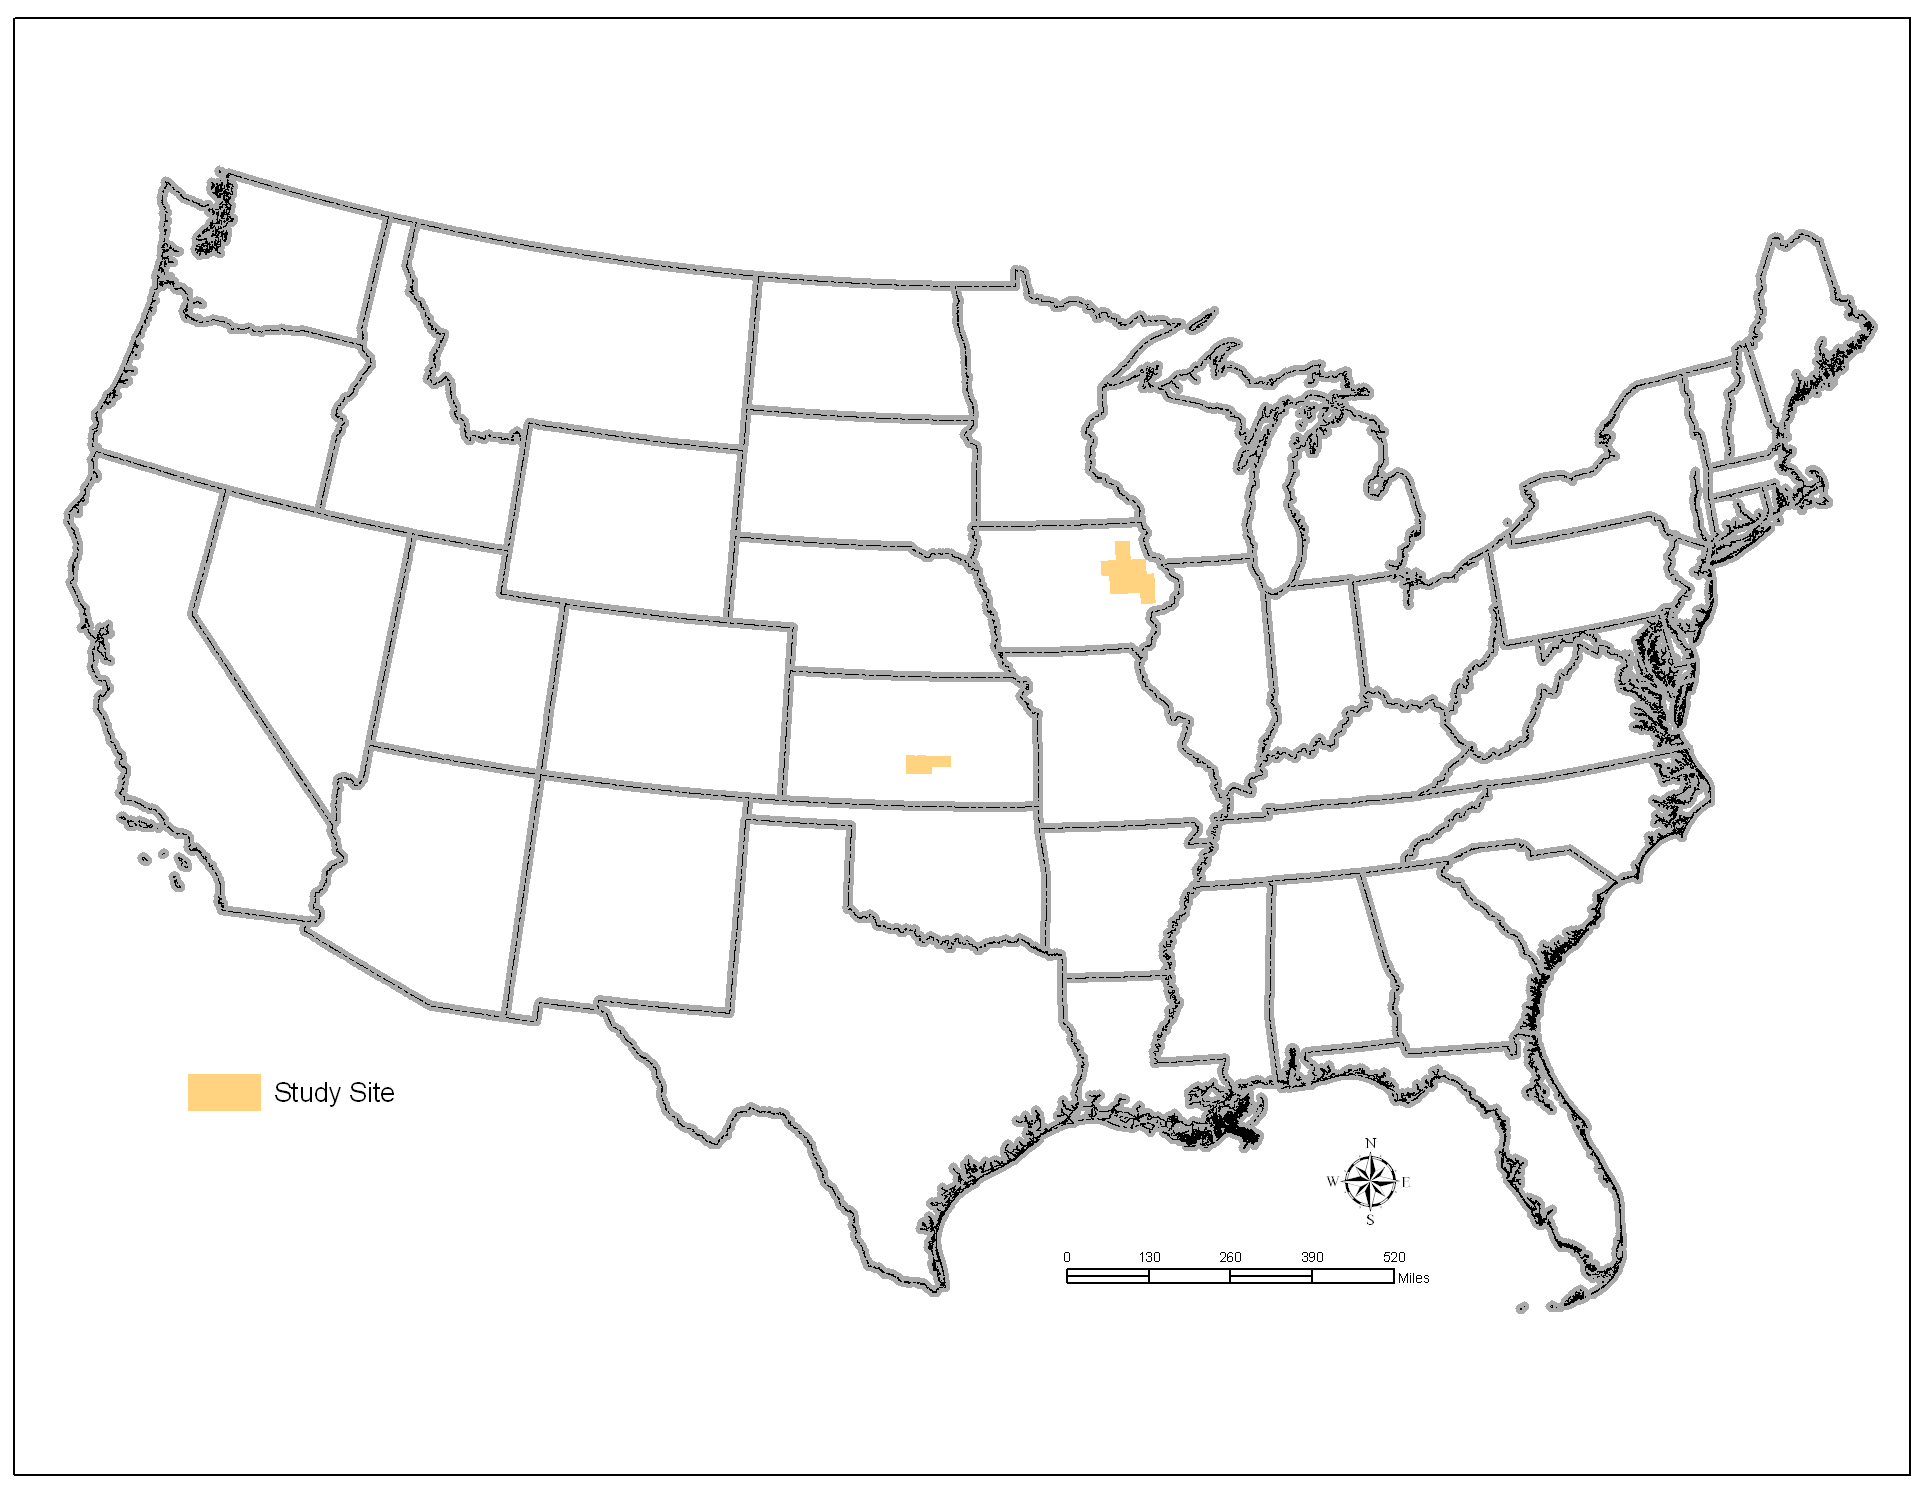
\includegraphics[width=1.0\textwidth]{iowa/study_site.png}  
%   \caption{Study Area}
%   \label{fig:study}
% \end{figure}


\begin{figure}[hpt]
  \centering
  \subfigure[Crop types]{
    \label{fig:crop}
    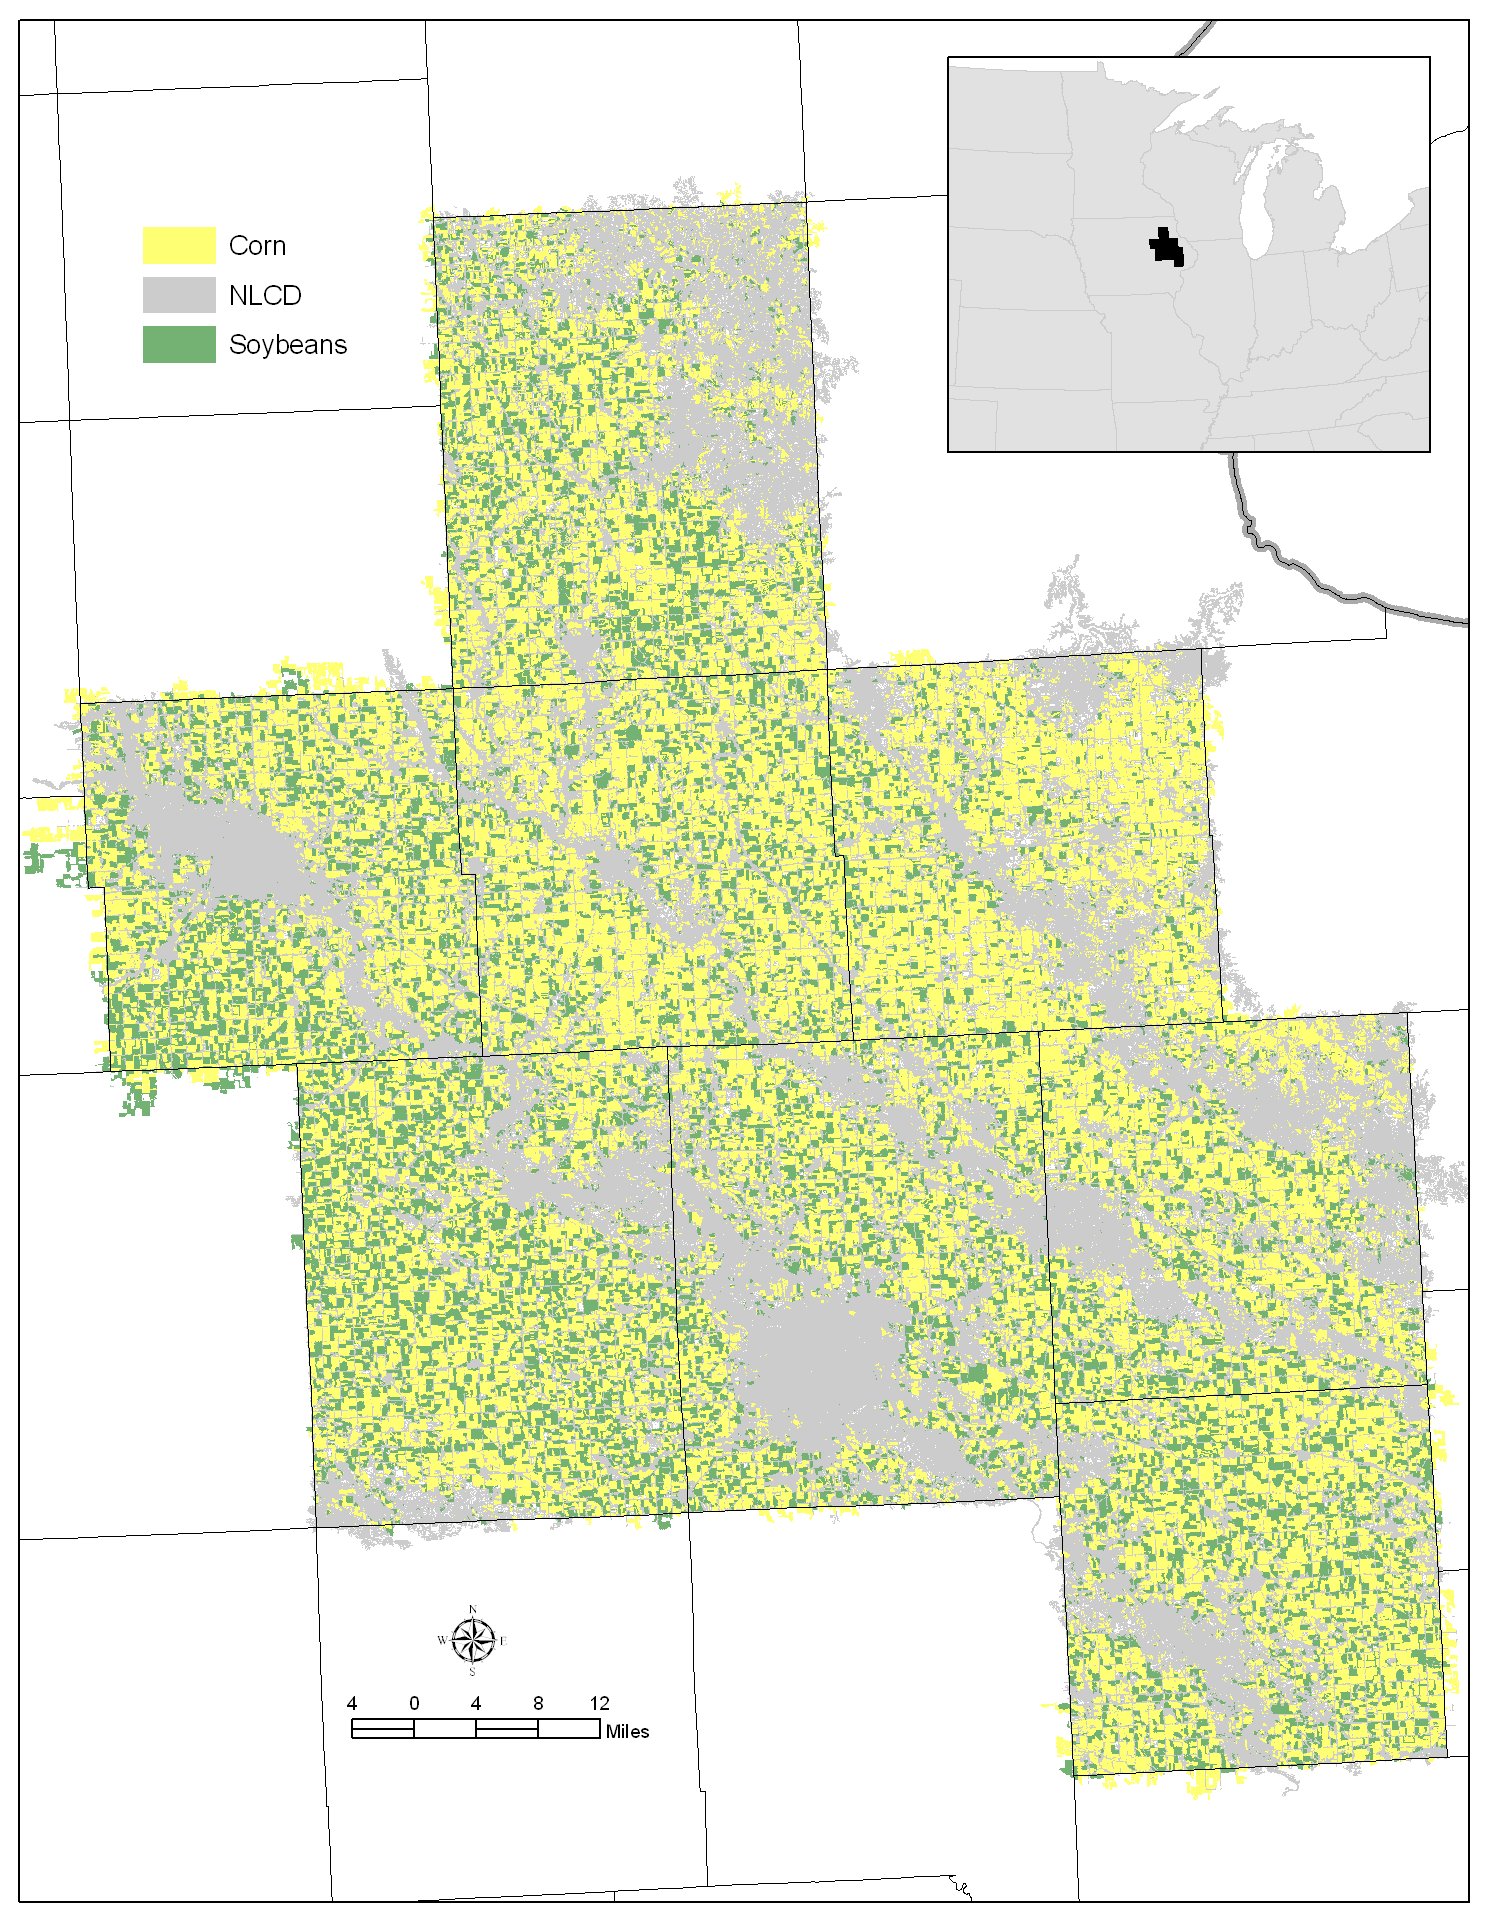
\includegraphics[width=0.45\textwidth]{iowa/crops_iowa.png}  
  }
  \subfigure[SSURGO Soils]{
    \label{fig:soil}
    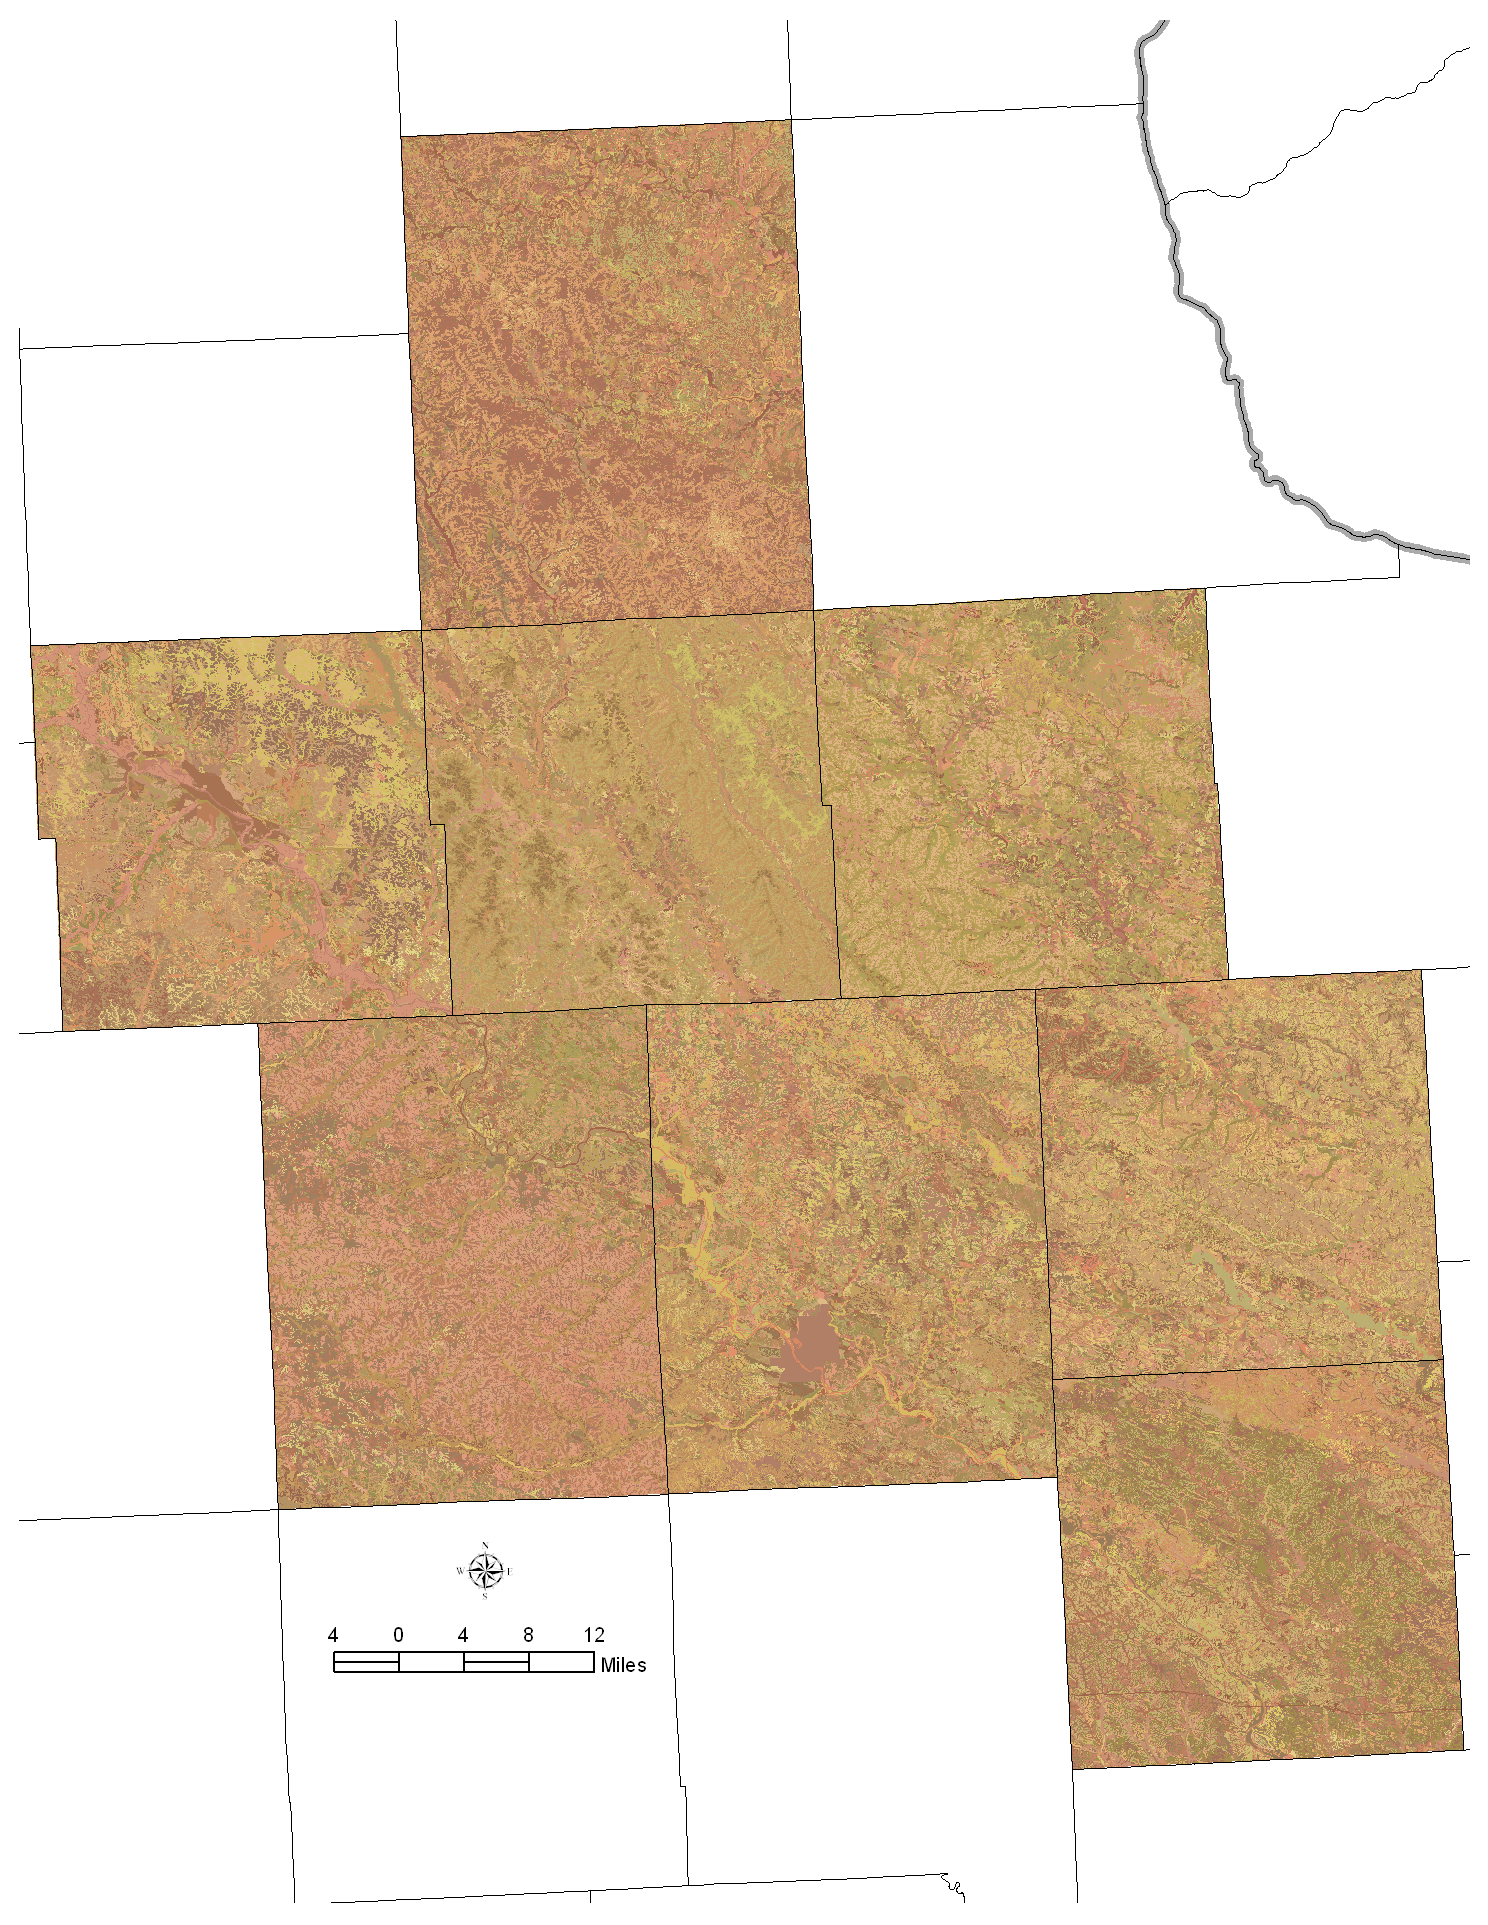
\includegraphics[width=0.45\textwidth]{iowa/ssurgo_iowa.png}  
  }
  \label{fig:study-area}  
  \caption{Study Area}
\end{figure}


\subsection{\ac{GIS} Model Development}
\label{sec:gis}

The purpose of the \ac{GIS} model for this program is to supply inputs
to the \ac{GAMS} optimization model.  These inputs include; the total
amounts of various feedstocks available; potential biorefinery
locations; transportation costs from feedstock sources to biorefinery
locations.

% Figure~\ref{fig:model} gives a notional overview of the \ac{GIS}
% model.  Figure~\ref{fig:network} shows the transportation connections
% between the various stages of the biofuel production.

% \begin{figure}[hpt]
%   \centering
% %  \includegraphics[width=\textwidth]{biofuels_network_v2}
%   \caption{\ac{GIS} Model Overview}
%   \label{fig:biofuels}
% \end{figure}


% \subsubsection{Network modeling}

% Roads marked code \emph{N} are not in the \ac{NHS} system, typically
% Rural and urban roads.  Roads in the database, but unmarked are
% considered local roads.

% \begin{table}[h]
%   \hrule\vspace*{2pt}
%   \caption{Road Travel Speed from \ac{NHPN}}
%   \centering
%   \begin{tabular}{clc}
%     \hline
%     Code & Route type & Speed \\ \hline
%     I &Interstate &65 \\
%     U &US Route &65 \\
%     S &Stae Route &55 \\
%     O &Off-Interstate Business Marker &45 \\
%     C &County Route &45 \\
%     T &Township &35 \\
%     M &Municipal &35 \\
%     P &Parkway or Forest Route Marker &15 \\
%     N &Rural and Urban roads &35 \\
%     \{\} & local roads &25 \\
%     \hline
%   \end{tabular}
%   \label{tab:road_speed}
% \end{table}


% \paragraph{Feedstock transportation costs}

% We have modeled biomass and liquid fuel transportation by two modes:
% trucking and rail.  The assumptions and references for the costs
% models are below.

% Trucking costs here are modeled with both time and distance
% dependence.  This differentiates the costs of traveling on slow local
% roads from fast highways.  The costs are listed in
% Table~\ref{tab:trucking} For fuel transportation, the insurance and
% permitting costs are doubled as the fuels are hazardous materials.

% \begin{table}[h]
%   \caption{Road Travel Speed from \ac{NHPN}}
%   \caption{Trucking Costs}
%   \centering
%   \begin{tabular}{lc}
%     \hline
%     Description & Cost \\
%     \hline
%     Biomass Loading & \unit[4.15]{\$} \\
%     Fuel Tanker Loading & \unit[2.24]{\$} \\
%     Labor & \unitfrac[18.81]{\$}{hr} \\
%     Capital (Biomass trucks) & 	\unitfrac[10.40]{\$}{hr}\\
%     Capital (Fuel tanker trucks) & \unitfrac[13.16]{\$}{hr}\\
%     Insurance &	\unitfrac[0.032]{\$}{km}\\
%     Licensing \& Permits & \unitfrac[0.035]{\$}{km}\\
%     Repairs and Maintenance & \unitfrac[0.206]{\$}{km}\\
%     Fuel & \unitfrac[0.469]{\$}{km}\\
%     \hline
%   \end{tabular}
%   \label{tab:trucking}
% \end{table}

% Biomass trucks have a payload of 25 wet tons.  The total cost is therefore 
% $C = 4.15+((18.81+10.40)/25)km/kmph+(0.035+0.206+0.4269)km$ or $C = 4.15+1.17m/mph+0.47m$.


% The cost for an individual feedstock source, $s$ to a particular
% biorefinery, $b$, is an function of the service area of the $s$, the
% distance from the source to the biorefinery, $d_{s,b}$, as well as.
% The value, $\frac{P_{s}}{8}$, based on the perimeter of the service
% area, is the average \emph{city-block}, distance with a feedstock
% source area, and is used to estimate transportation costs with a
% feedstock source area.

% % For the current implementation, the individual costs associated with
% % preparation and intra-source and extra-source transportation are
% % considered constant with respect to the feedstocks and are shown in
% % Table~\ref{tab:feedstock_costs}.

% % \begin{table}[htbp]
% %   \hrule\vspace*{2pt}
% %   \caption{Feedstock Transportation Cost Constants}
% %   \centering
% %   \label{tab:feedstock_costs}
% %   \begin{tabular}{l|l|l}
% %     Cost Item & Description & Cost \\
% %     \hline \hline
% %     \acs{Uitrf} & \acl{Uitrf} & \unitfrac[0.25]{\$}{bdt\,mi} \\
% %     \acs{Uxtrf} & \acl{Uxtrf} & \unitfrac[0.25]{\$}{bdt\,mi} \\
% %     \acs{Upf} & \acl{Upf} & \unitfrac[1]{\$}{bdt} \\ 
% %   \end{tabular}
% % \end{table}


\section[Implementation]{Feedstock modeling}


Figure~\ref{fig:overview} shows a basic overview for determining the
variation on harvest yield for an agricultural region.  The process
involves dividing the region in to representative pseudo farms, deciding
on whether these farms are in production based on a land cover map,
and then assigning variable yields based on the county estimates and
underlying soil types.

\begin{figure}[hpt]
  \centering
  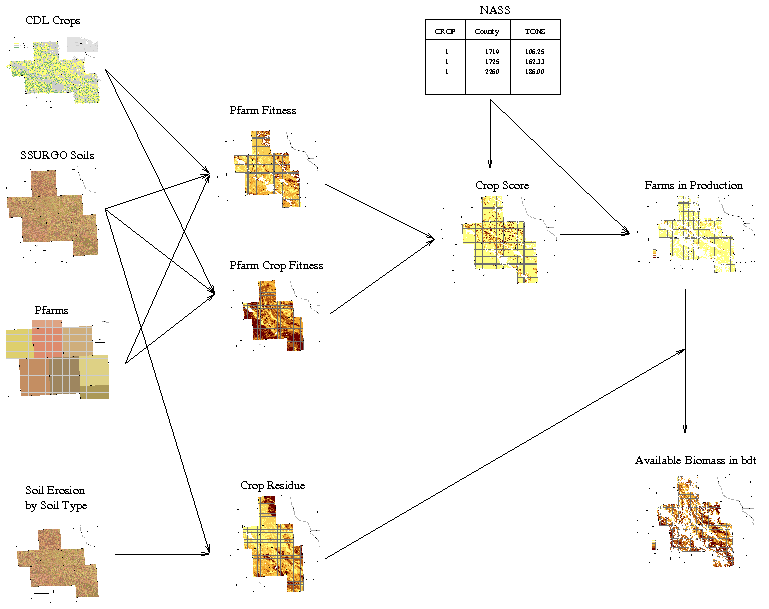
\includegraphics[width=0.75\textwidth]{iowa/maps.png}  
  \caption{Overview}
  \label{fig:overview}
\end{figure}

\subsection{Pseudo-farms}

First, the region is divided into a series of \emph{pseudo-farms}
(Figure~\ref{fig:pfarms}).  These are matched to a standard grid as
opposed to trying to match any real farm delineations.  A standard grid
is chosen to provide some faster image processing for some national
level datasets, like land cover for example.  Pseudo-farms are needed
to divide the area into workable sizes.

For each pseudo-farm, a number of fitness variables are assigned, to
try and determine where crops will be grown, and their yields.

\emph{Farm fitness}~(Figure~\ref{fig:fitness}), is a score without a
specific crop which gives the total amount of arable land and the
average land capability.  Farms need to be more then 10\% arable to be
included.  Otherwise it is considered not farmed.

For a specific crop, \emph{Pseudo-farm crop
  fitness}~(Figure~\ref{fig:crop-fitness}), calculates the amount of
area either identified as that crop, or identified as typical crop for
the underlying soil types.  Also calculates expected yield for crop.
  
%    \begin{lstlisting}
% pfarm_gid | crop_id | nass_area | ssurgo_area |      irr_yield      %
%
%     68508 |       2 |    314336 |      999991 | 75.0000000000000000 
%     68600 |       2 |     61125 |      819427 | 69.4461538461538462 
%     68602 |       2 |     64652 |     1000000 | 75.0000000000000000 
%     68603 |       2 |     84127 |     1000000 | 75.0000000000000000 
%     68604 |       2 |    147789 |      999833 |                     
%    \end{lstlisting}


The \emph{Farm crop score} combines NASS cropland types and SSURGO
fitness, for the crop and in general.  Areas with both get scored
highest.


\begin{figure}[hpt]
  \centering
  \subfigure[Pseudo-farms]{
    \label{fig:pfarms}
    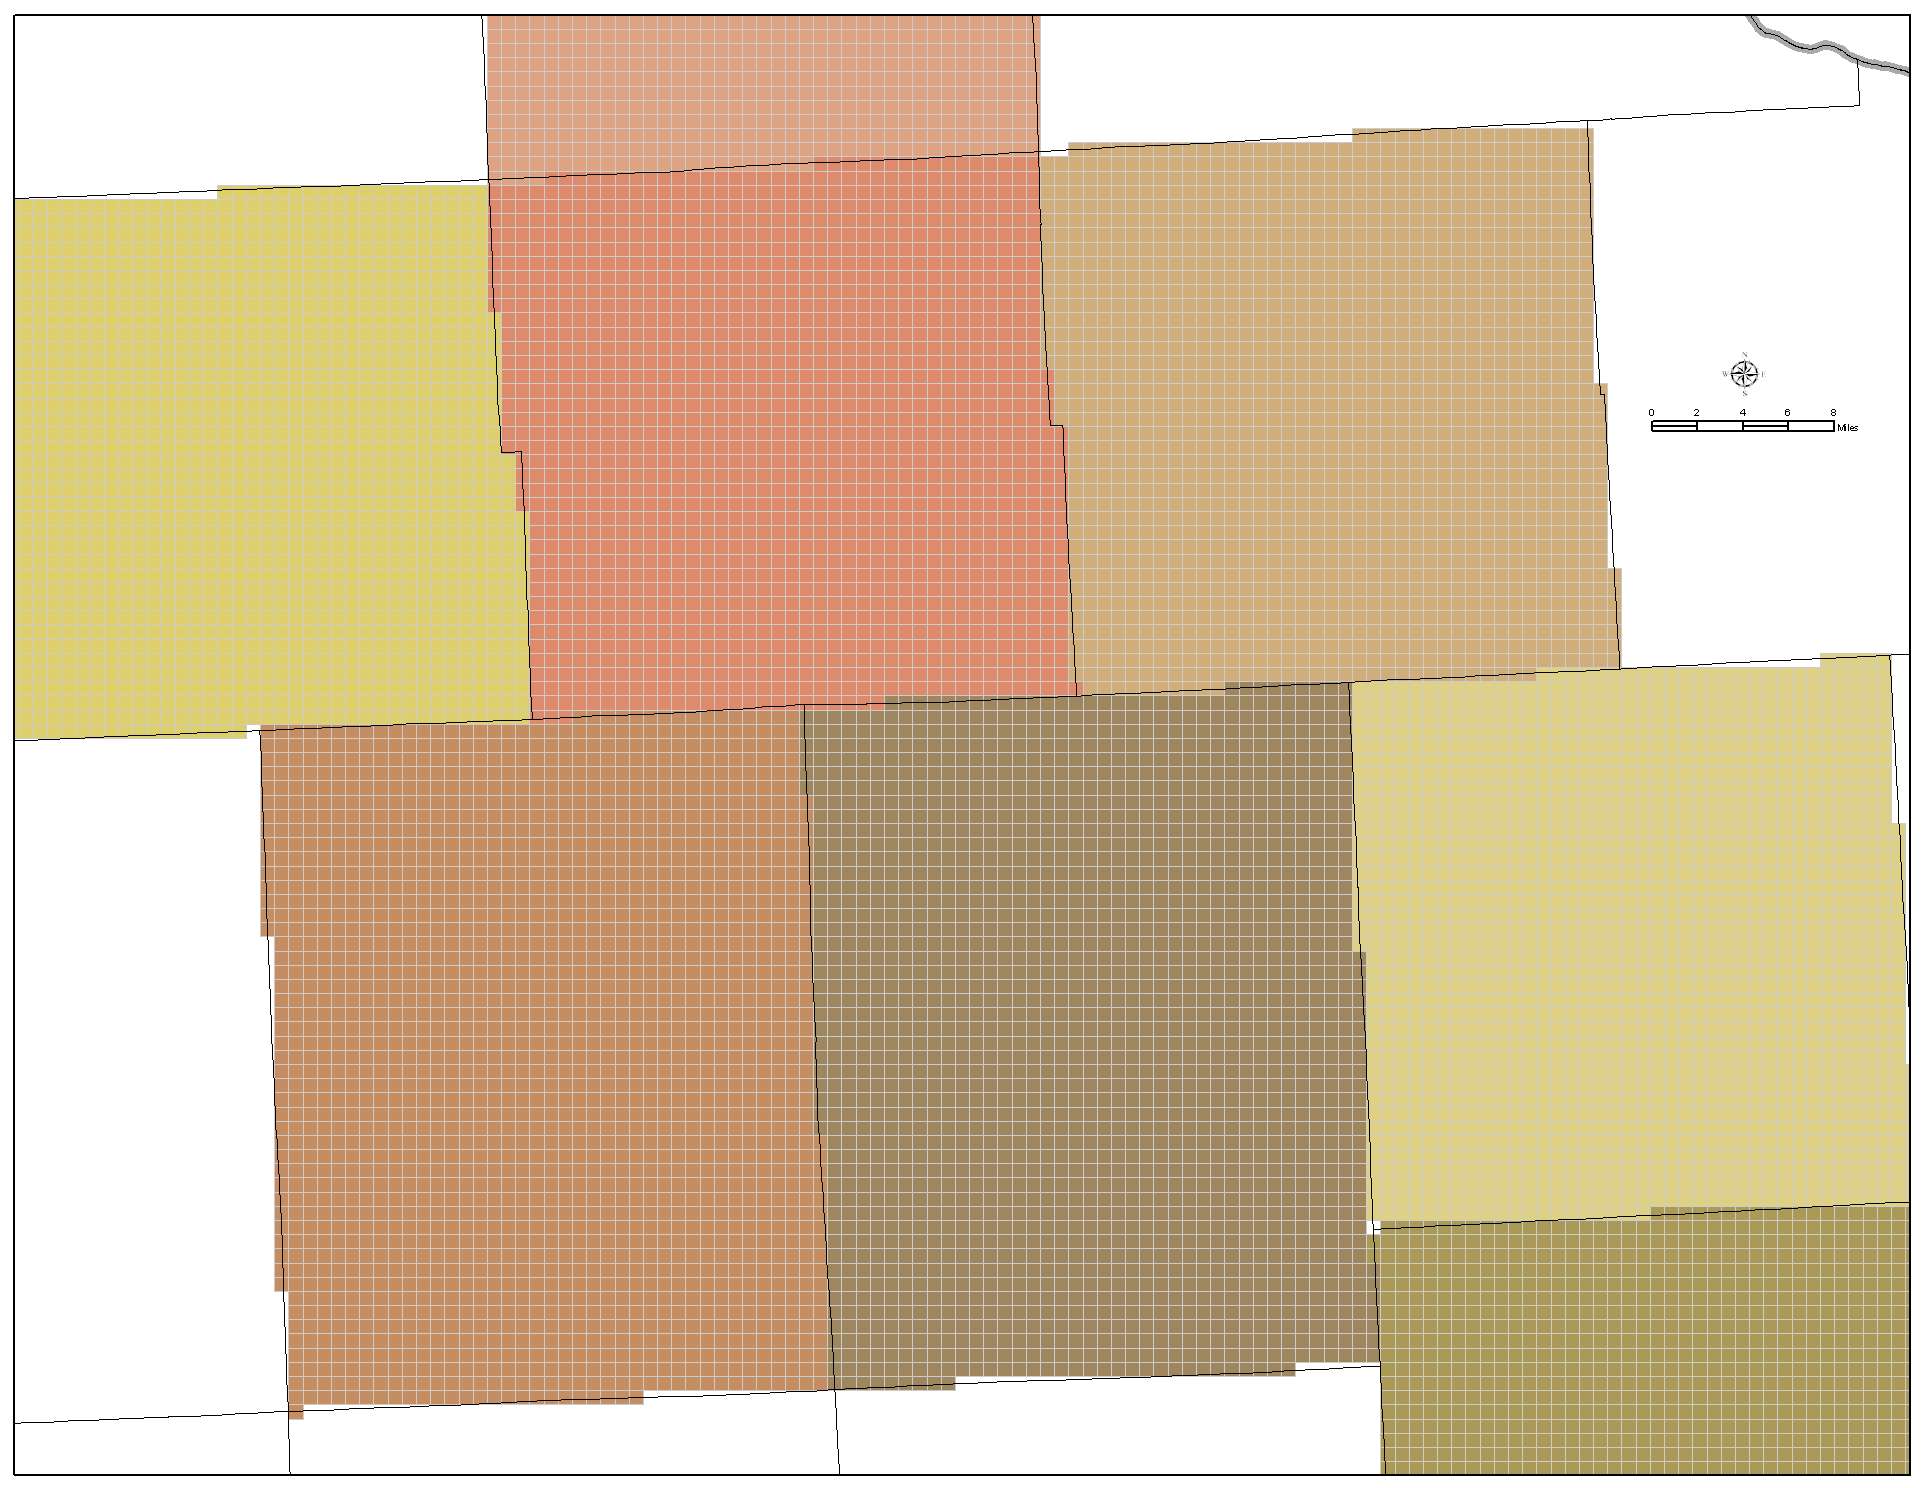
\includegraphics[width=0.45\textwidth]{iowa/pfarms.png}
  }
  \subfigure[Pseudo-farm fitness] {
    \label{fig:fitness}
    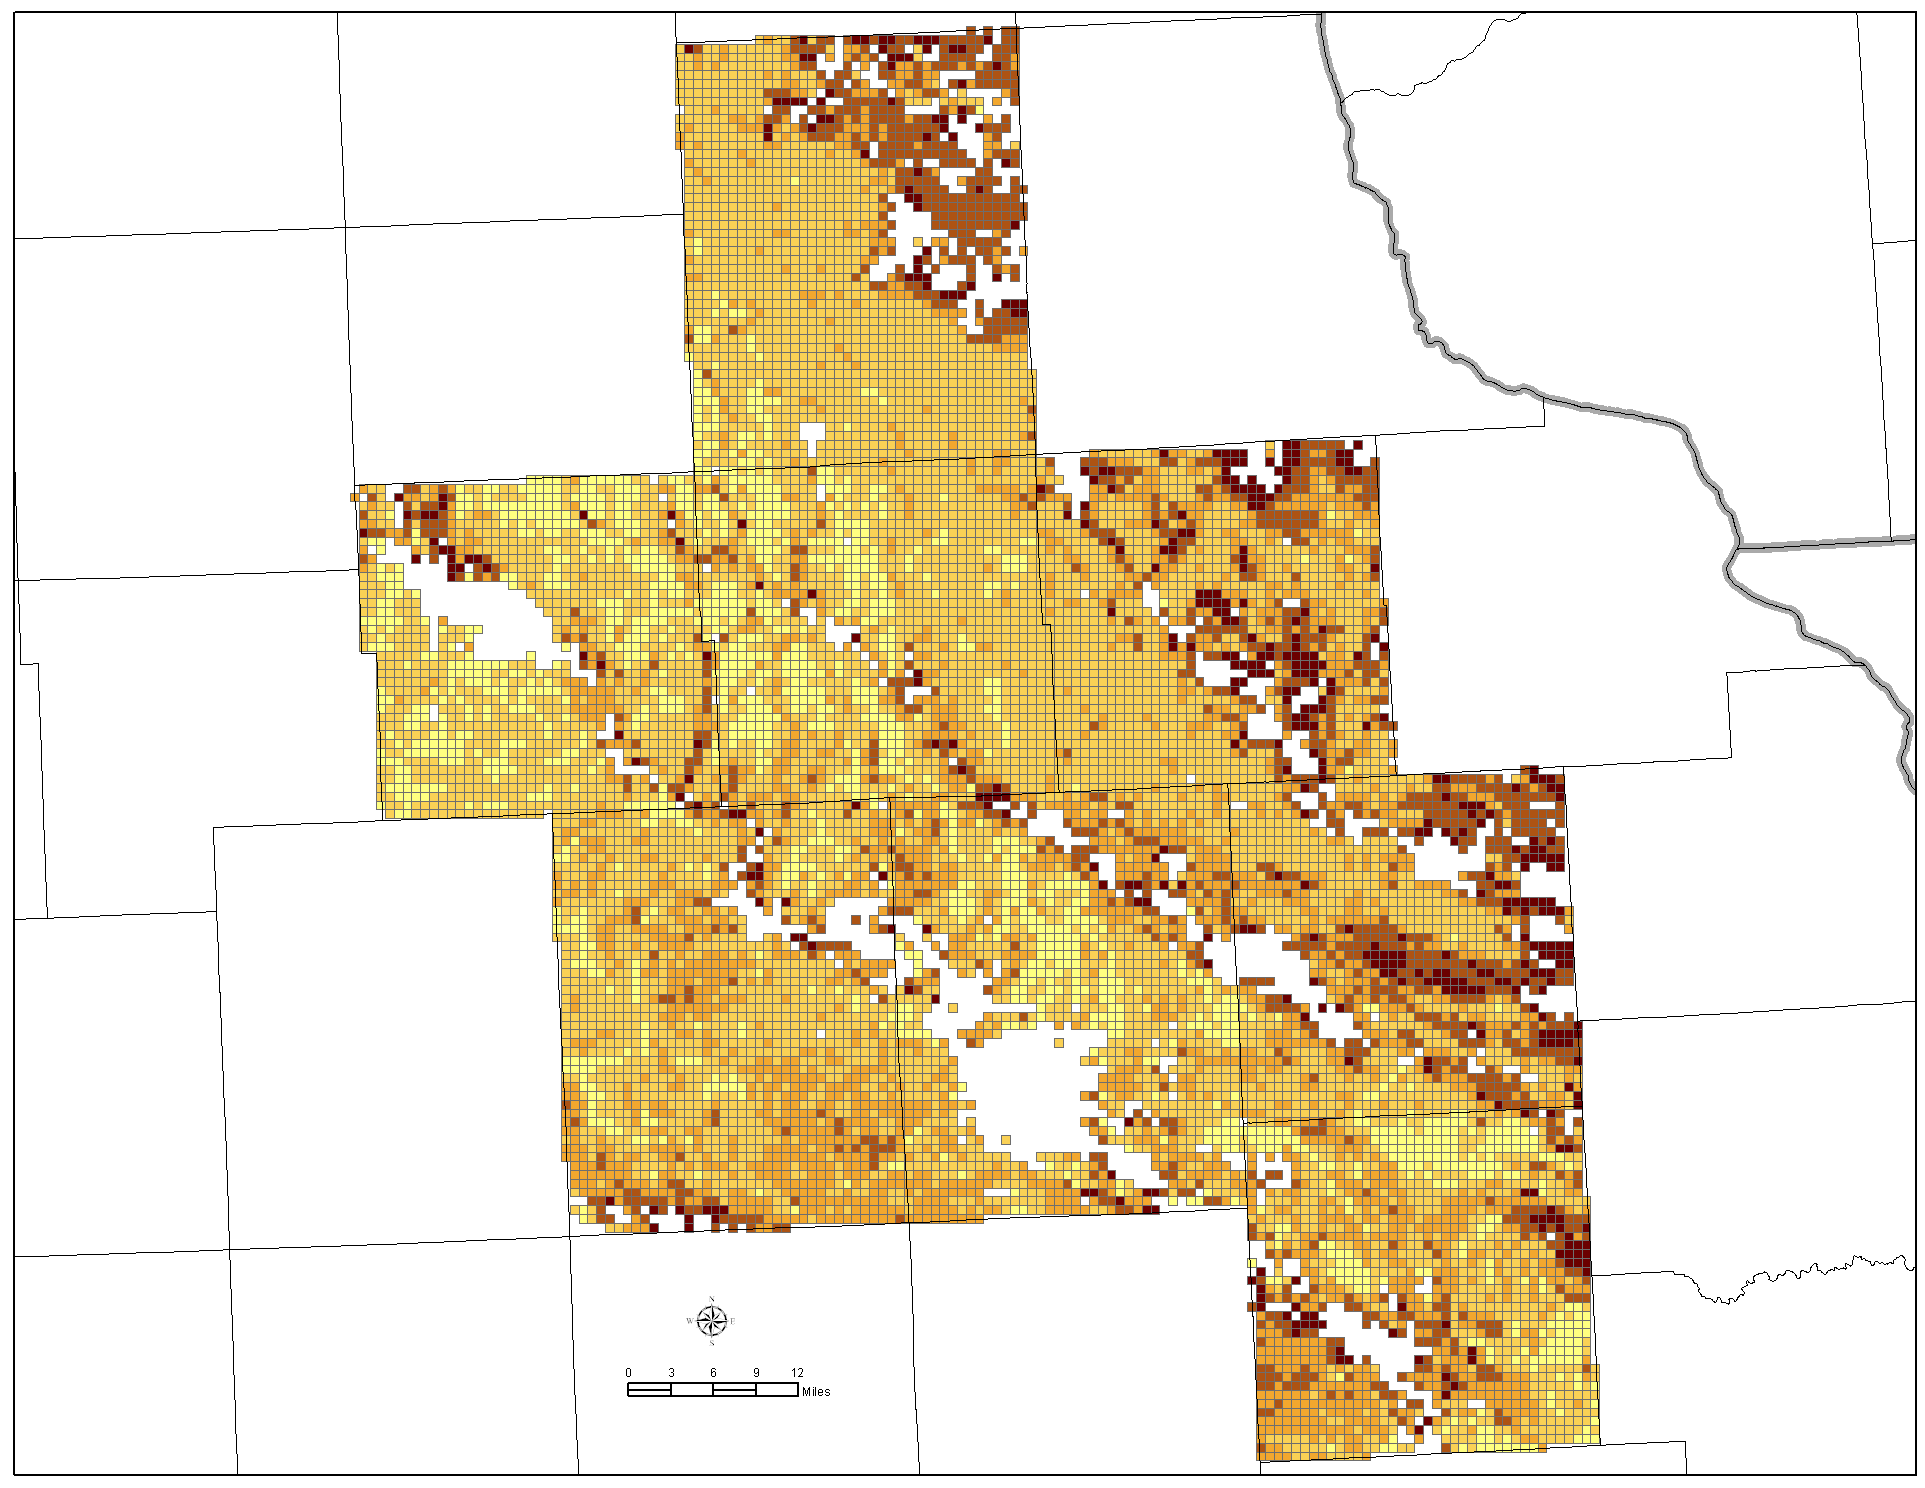
\includegraphics[width=0.45\textwidth]{iowa/pfarms_fitness.png}  
  }

  \subfigure[Pseudo-farm crop fitness]{
    \label{fig:crop-fitness}
    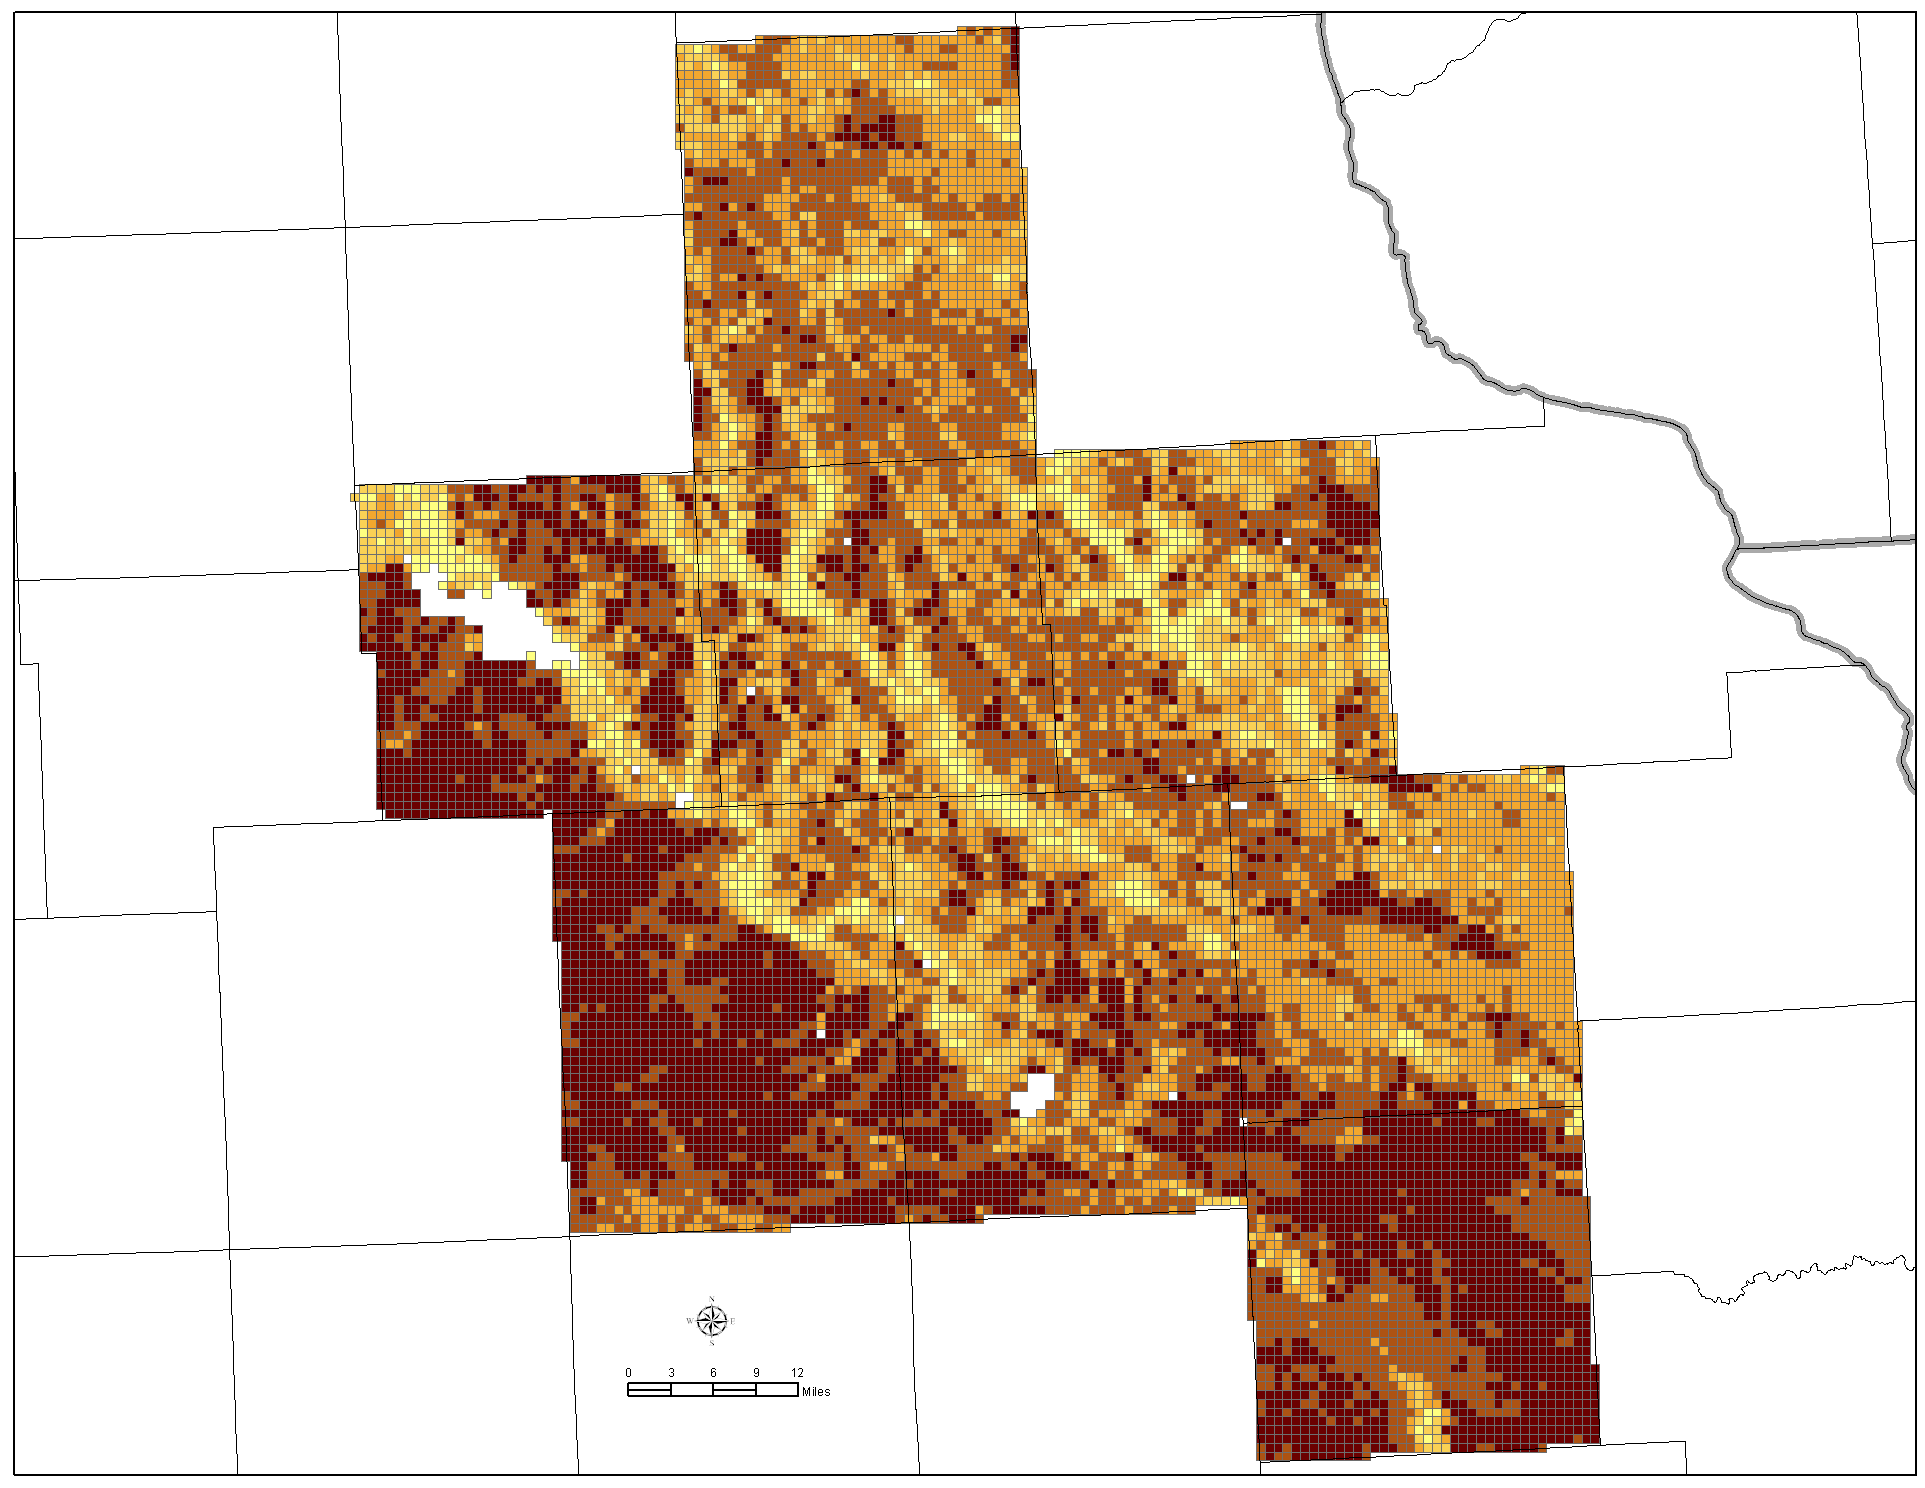
\includegraphics[width=0.45\textwidth]{iowa/pfarms_crop_fitness.png}  
  }
  \subfigure[Pseudo-farms Score] {
    \label{fig:scoring}
    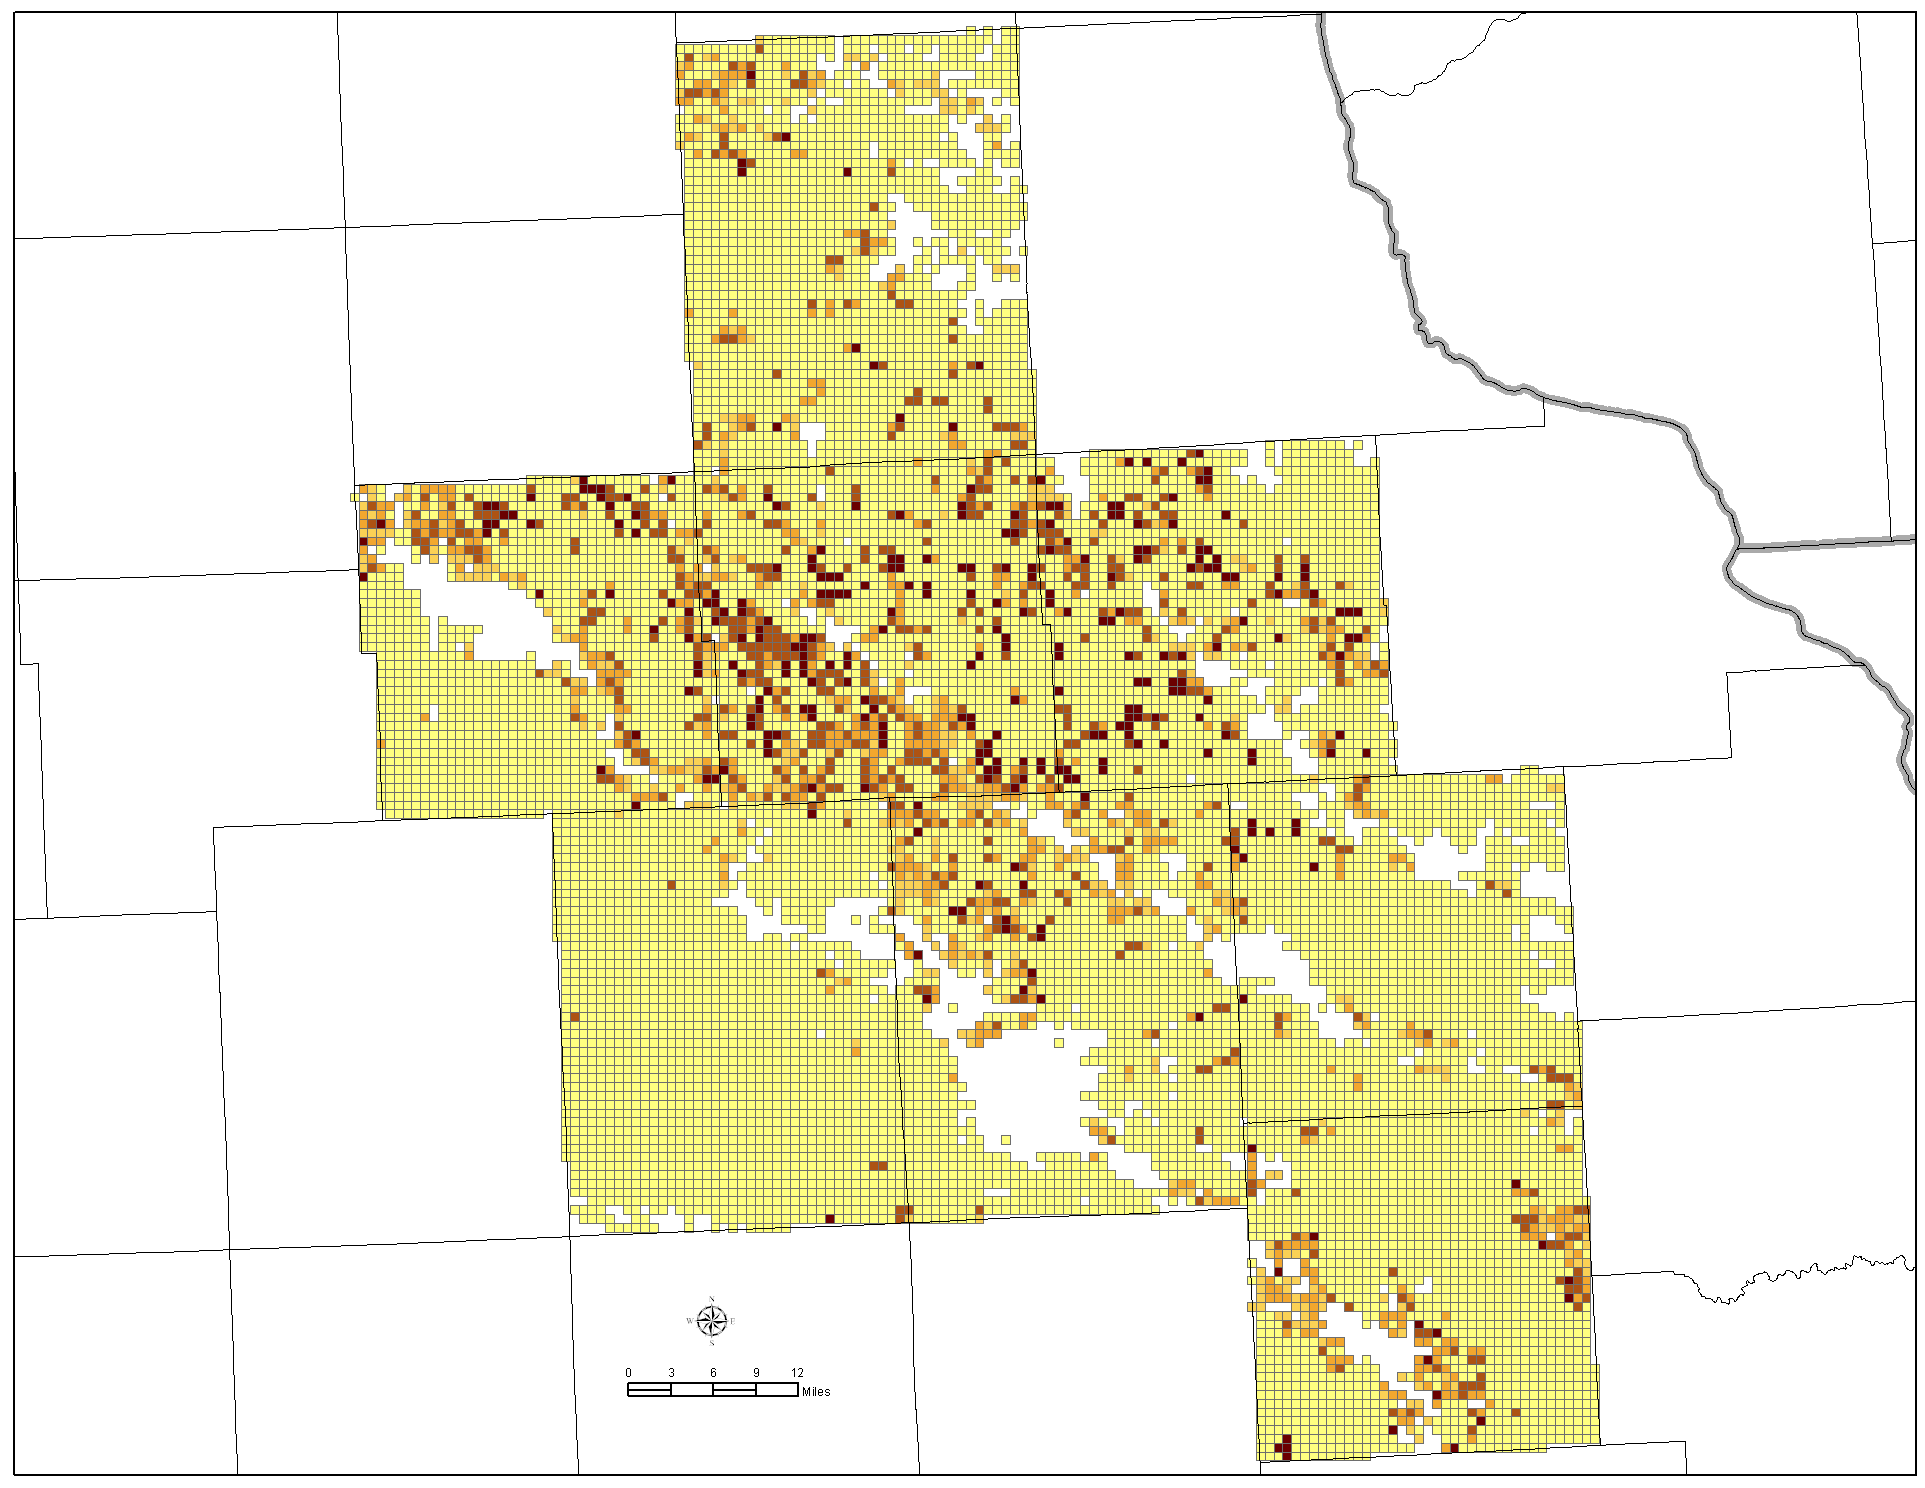
\includegraphics[width=0.45\textwidth]{iowa/pfarms_crop_score.png}  
  }
  \label{fig:scores}
  \caption{Pseudo-farm scoring}
\end{figure}


Now for a particular crop type and expected acres harvested the most
likely pseudo-farms to be planted are selected. Actual, per-county
production amounts are used to get pseudo-farms in production for a
specific year.  Once the farms are selected, we adjust the yields
within the farms to match the total county output. Use an average
yield for soils without crop yields (Figure~\ref{fig:actual}.

Once yields are calculated, the amount of biomass recovered needs to
be determined. Each pseudo-farm has a soil type and slope that affects
how much residue needs to be left on for tolerable soil
loss~(Figure~\ref{fig:biomass}).

Use the bushels of predicted corn to estimate the standing biomass,
and remove the residue needed, to produce a map of standing biomass
per pseudo-farm~(Figure~\ref{fig:actual-bio}).


\begin{figure}[hpt]
  \centering
  \subfigure[Pseudo-farms in Actual Production]{
    \label{fig:actual}
    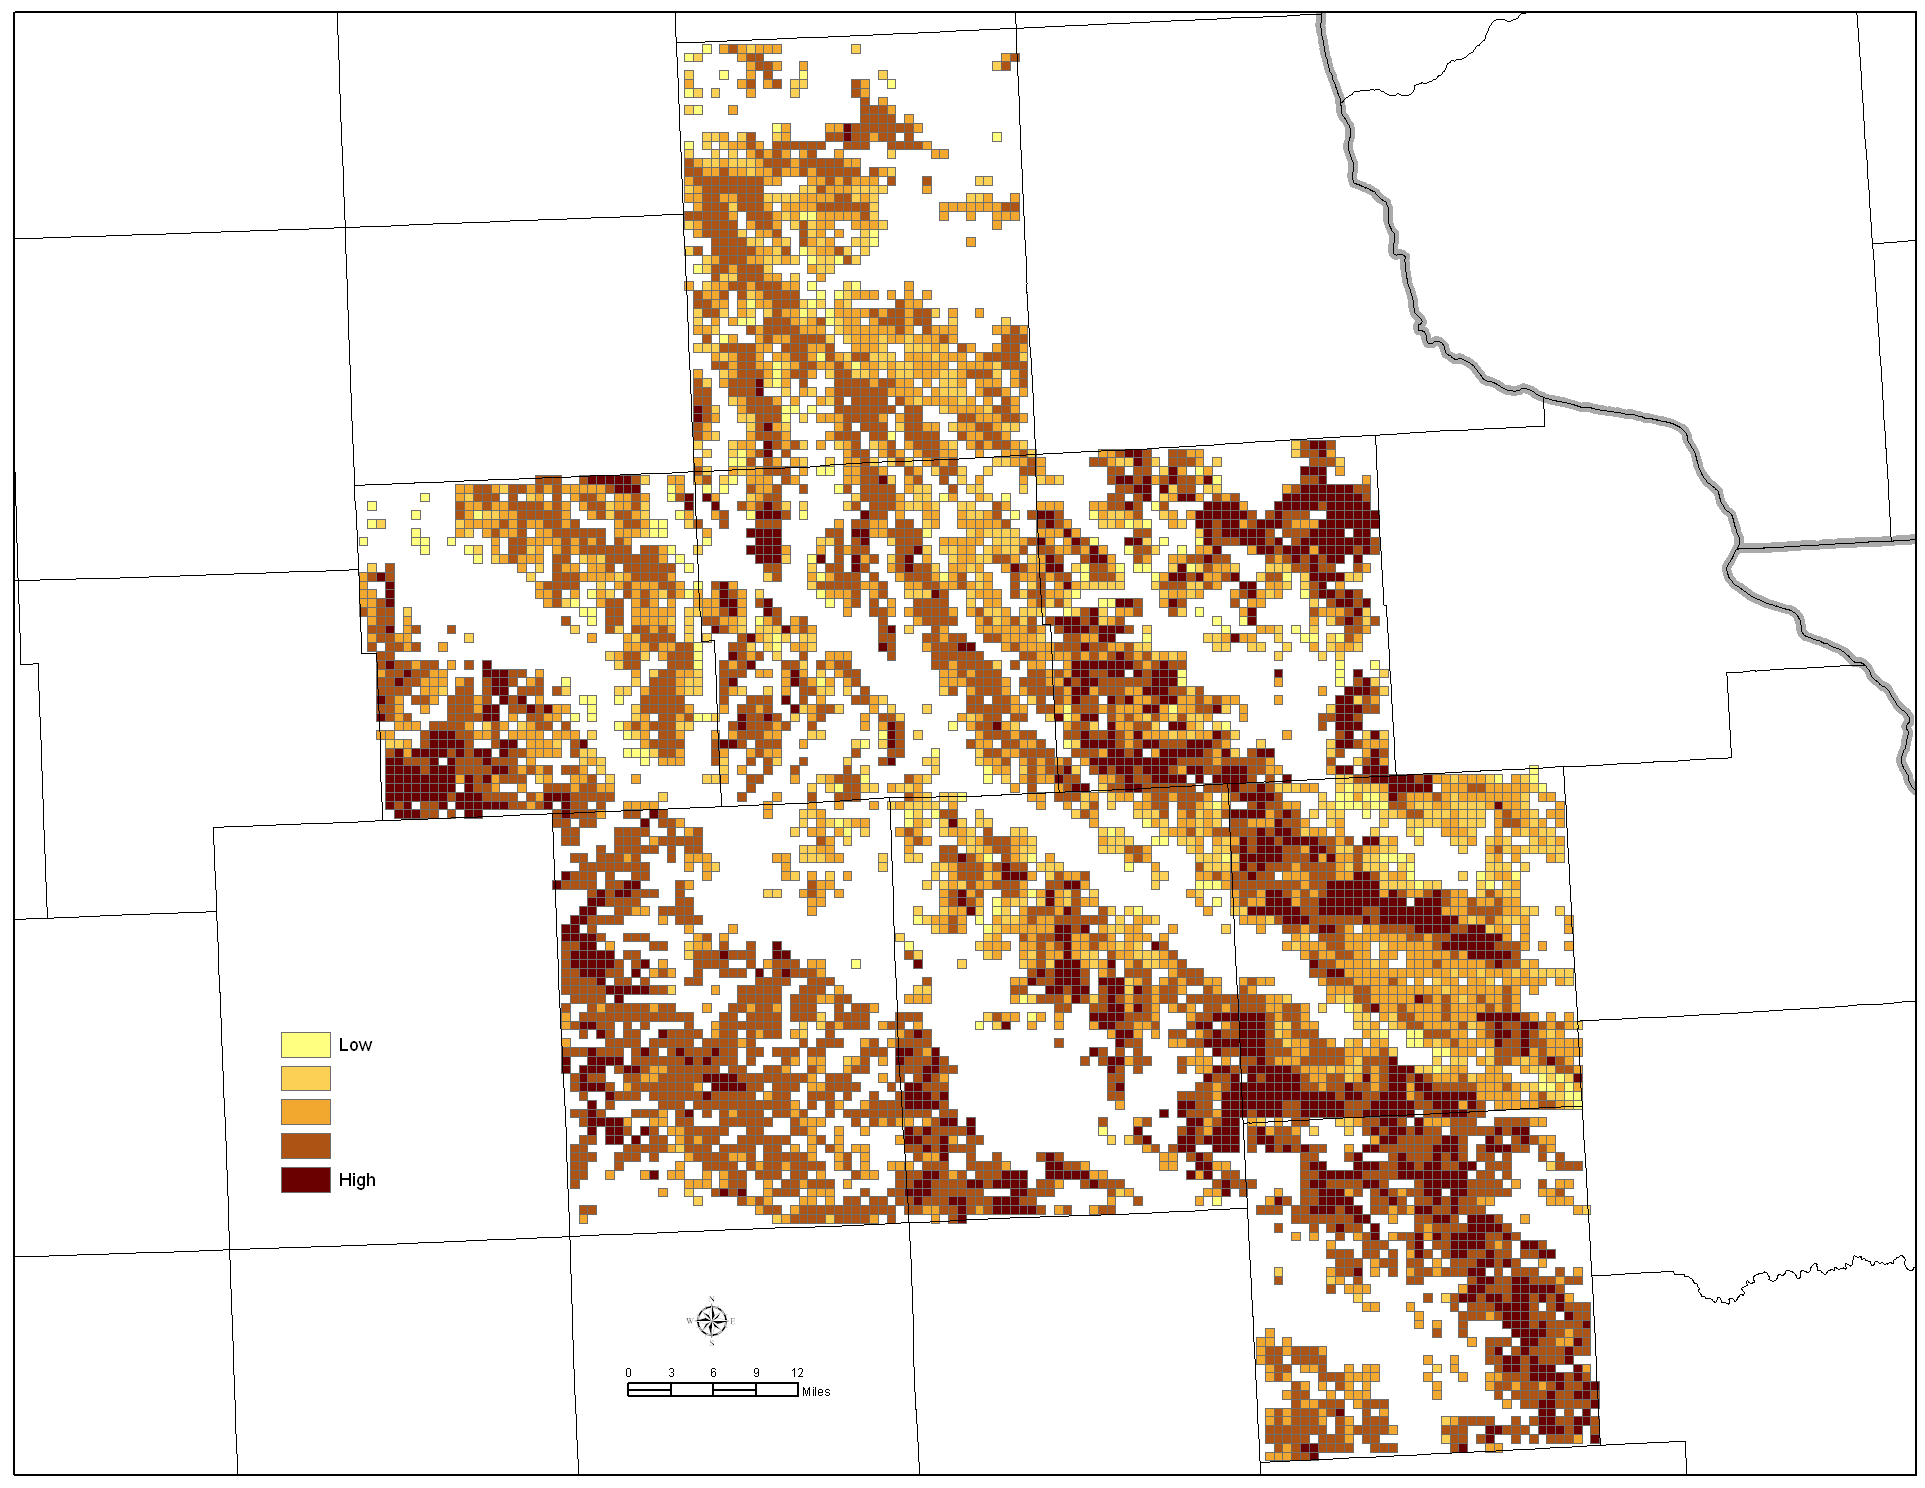
\includegraphics[width=0.45\textwidth]{iowa/m_pfarms_actual_production.png} 
  }
  \subfigure[Crop residues] {
    \label{fig:biomass}
    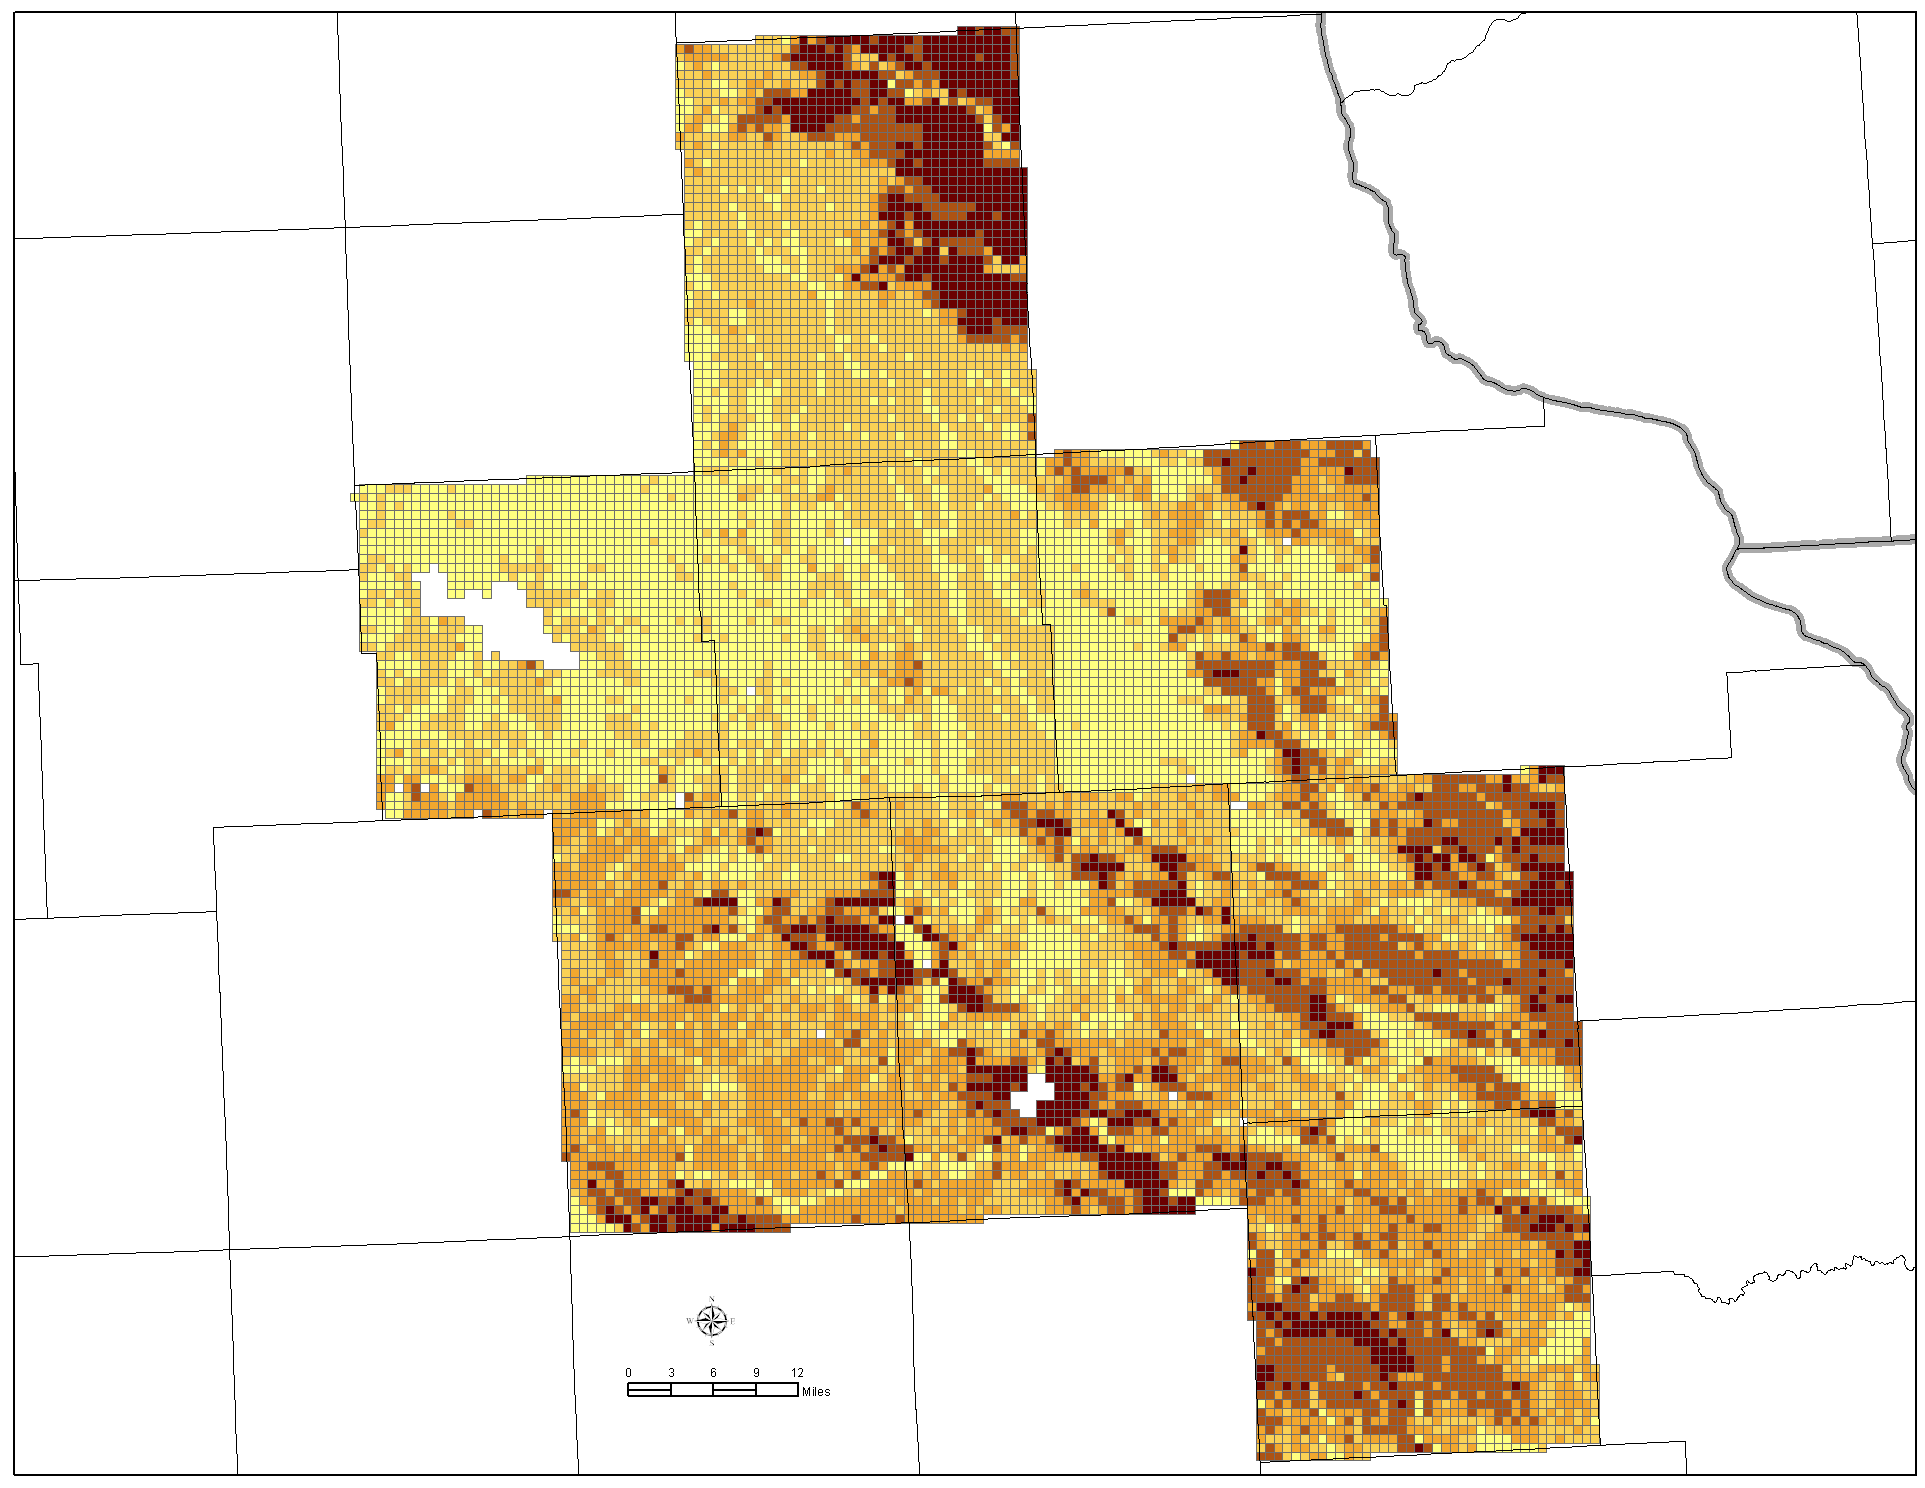
\includegraphics[width=0.45\textwidth]{iowa/pfarms_crop_residue.png}  
  }
  \subfigure[Pseudo-farm yields] {
    \label{fig:actual-bio}
    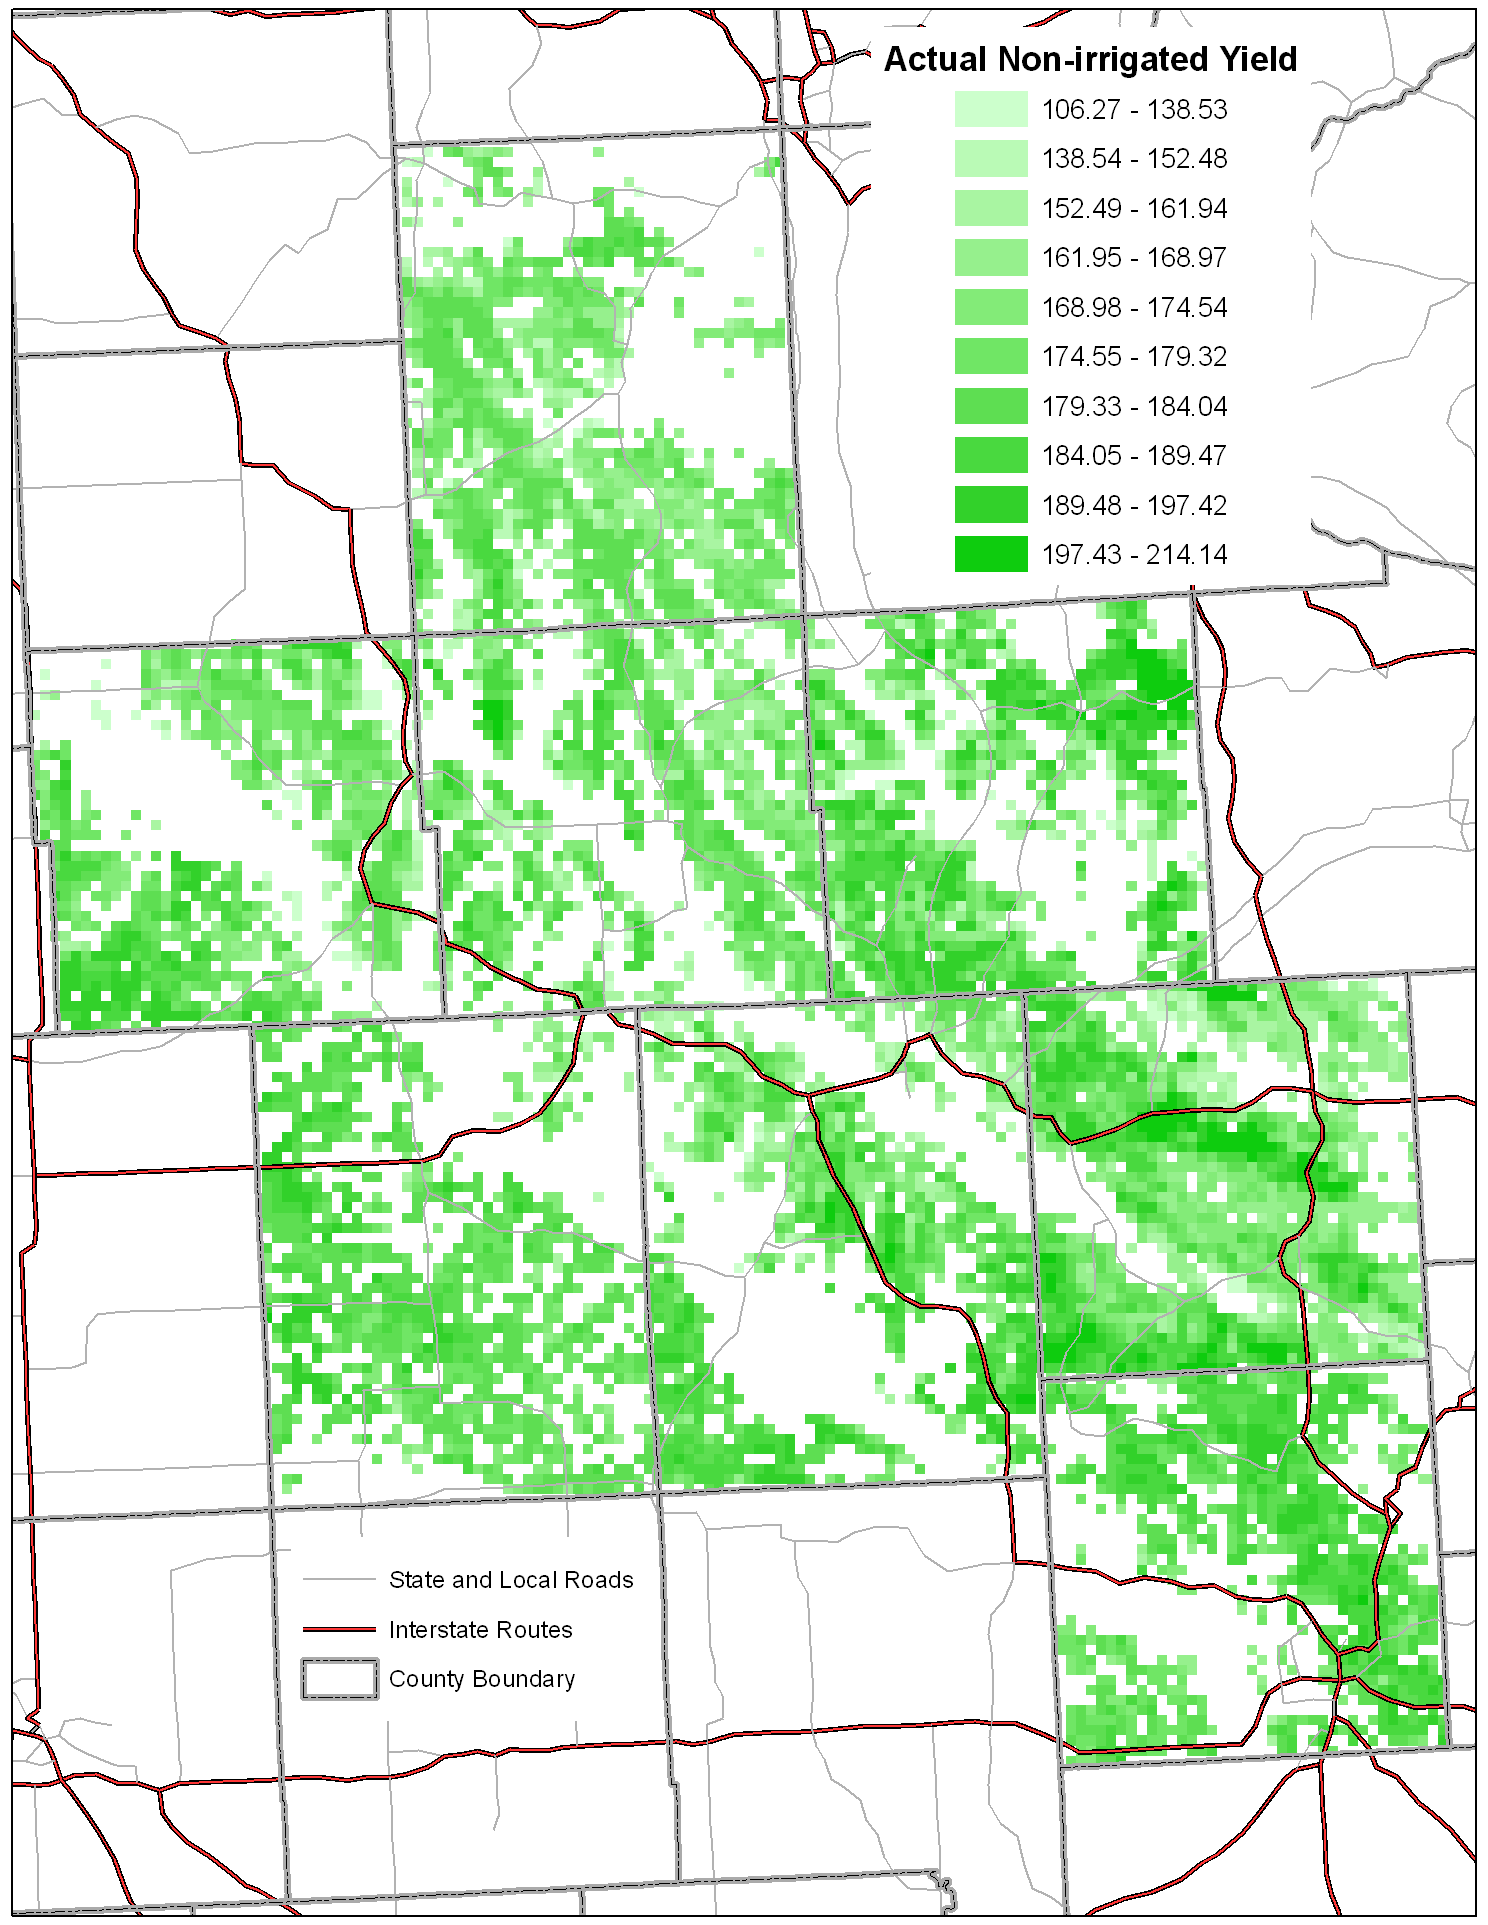
\includegraphics[width=0.45\textwidth]{iowa/farm_costs_nonirr_yield.png}  
  }
  \label{fig:biomass}
  \caption{Pseudo-farm biomass}
\end{figure}


\section{Results}

Eight counties were modeled in this study.  From the total amount of
biomass available from these counties, four refineries were located to
process the biomass.  The refineries were located using a k-means
clustering on the total amount of feedstock, as a method of
approximating equally sized refineries.

Figure~\ref{fig:destination} shows location of the refineries and the
expected destination of the feedstock for each refinery.  This model
is the result of running a network model that includes all roads
within the region, and assigning each pseudo-farm to the refinery
closest to it.  The map shows that despite this more accurate
networking model, feedstocks generally are assigned to the most
geometrically proximate feedstock location.  Also, when refineries
utilize all feedstock, then the feedstock ``sheds'' of the refineries
are necessarily well modeled as circular patterns. 

Figure~\ref{fig:travel} shows a breakdown of the actual travel costs
associated with the individual pseudo-farms within a refinery
region. These costs only include the on-road time costs, and do not
include farmgate, loading, or unloading costs.  As will be seen, this
contributes most to the variation in the supply curves for feedstock
availability.

\begin{figure}[hpt]
  \centering
  \subfigure[Representative Refinery locations and their associated feedstock sheds] {
    \label{fig:destination}
    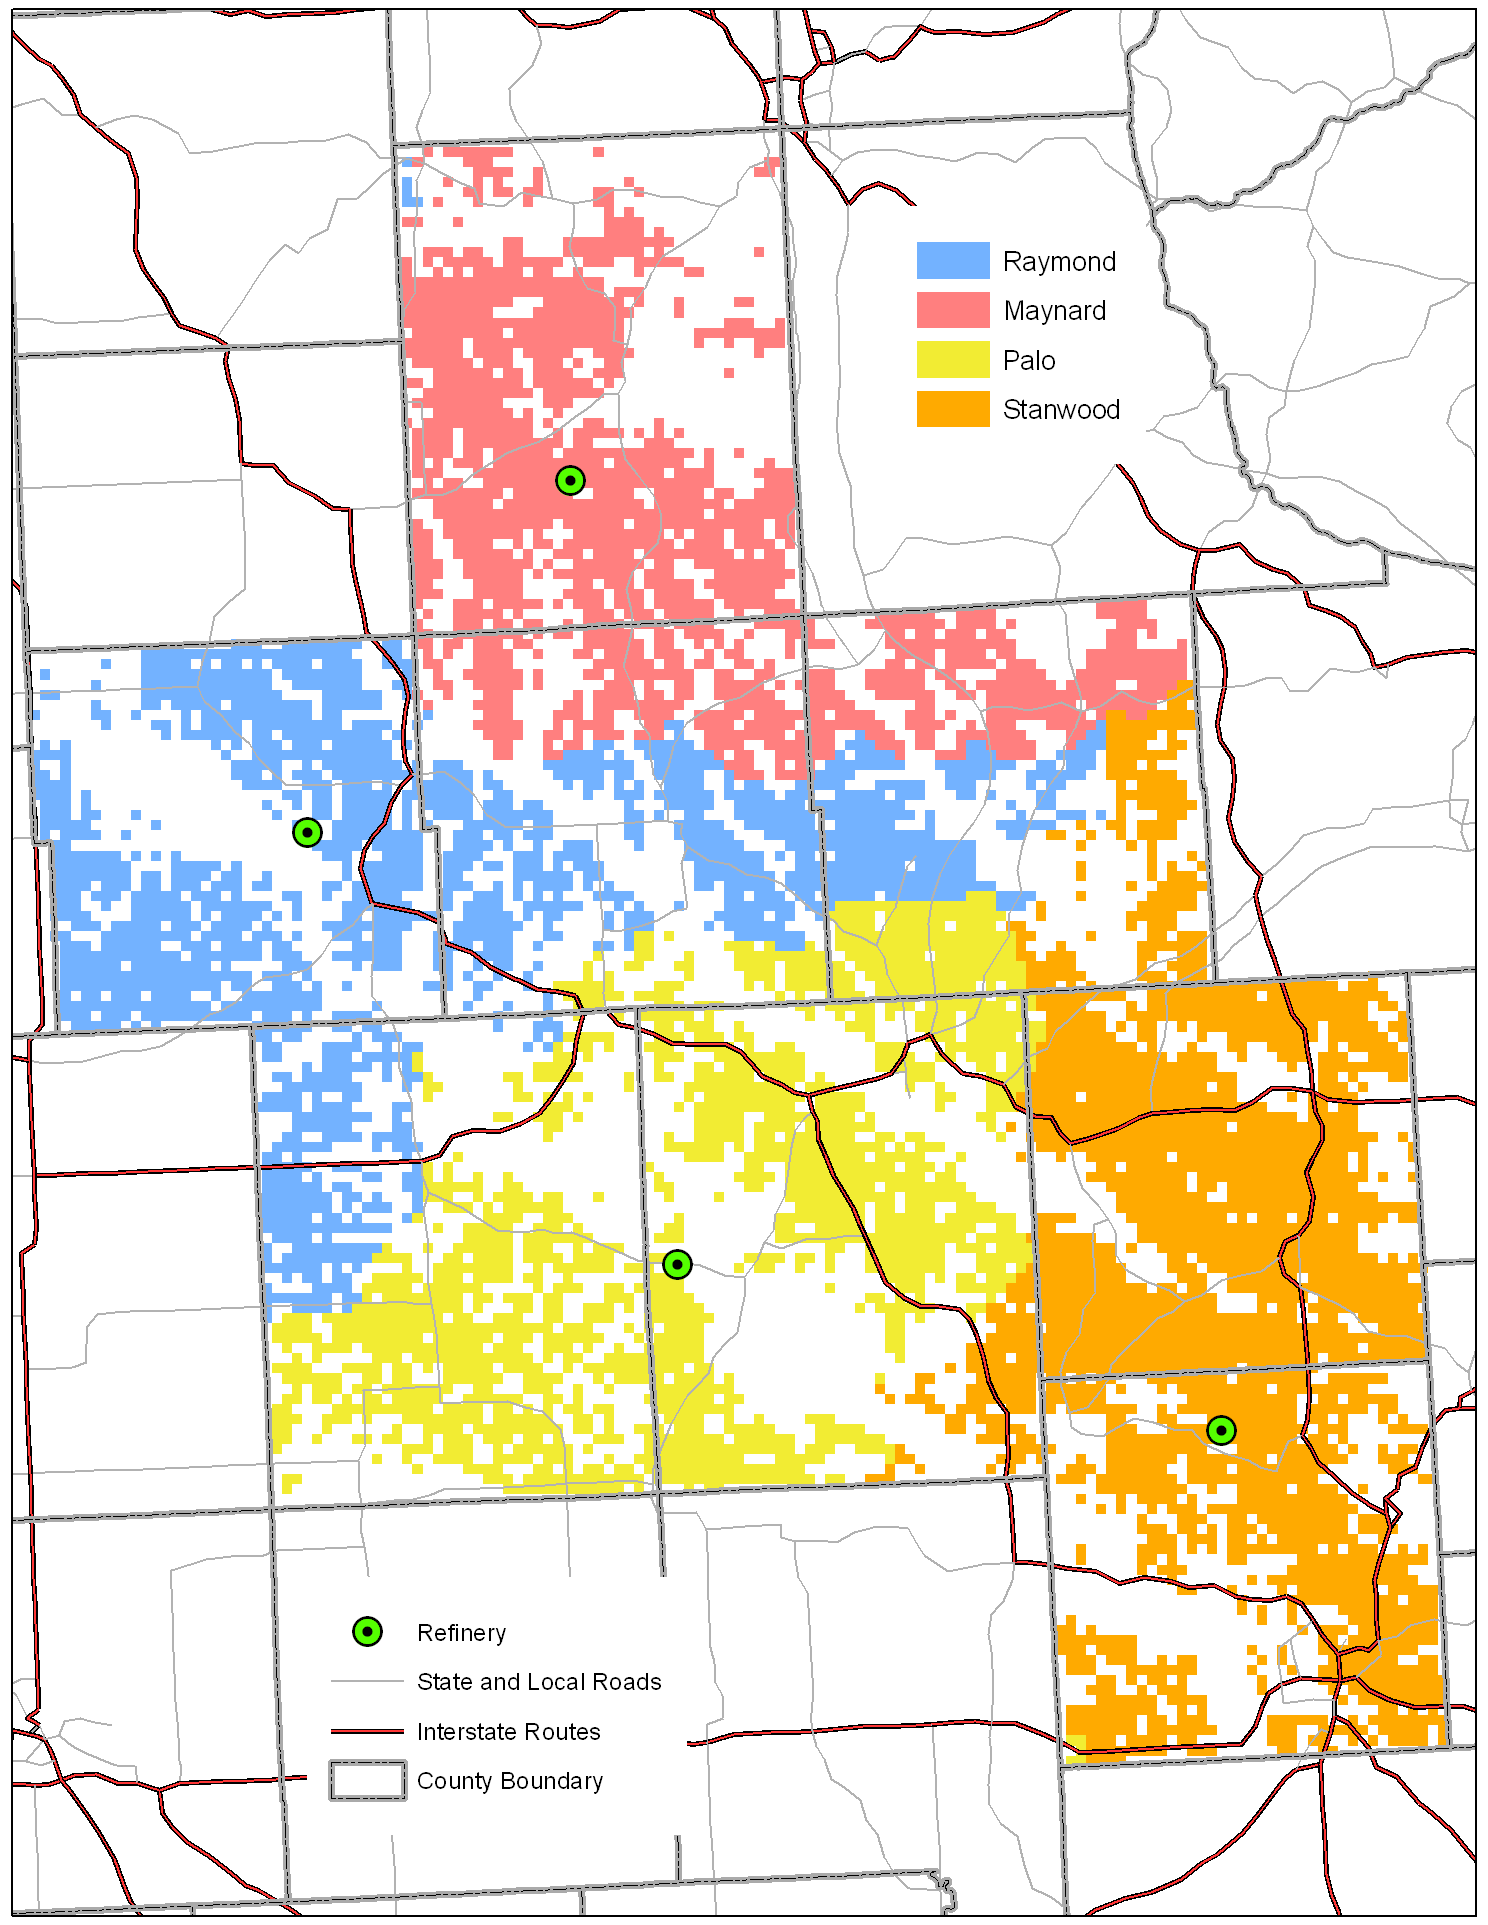
\includegraphics[width=0.45\textwidth]{iowa/farm_costs_destination.png}  
    }
    \subfigure[Travel costs \unitfrac{\$}{bdt} for individual farms] {
      \label{fig:travel}
      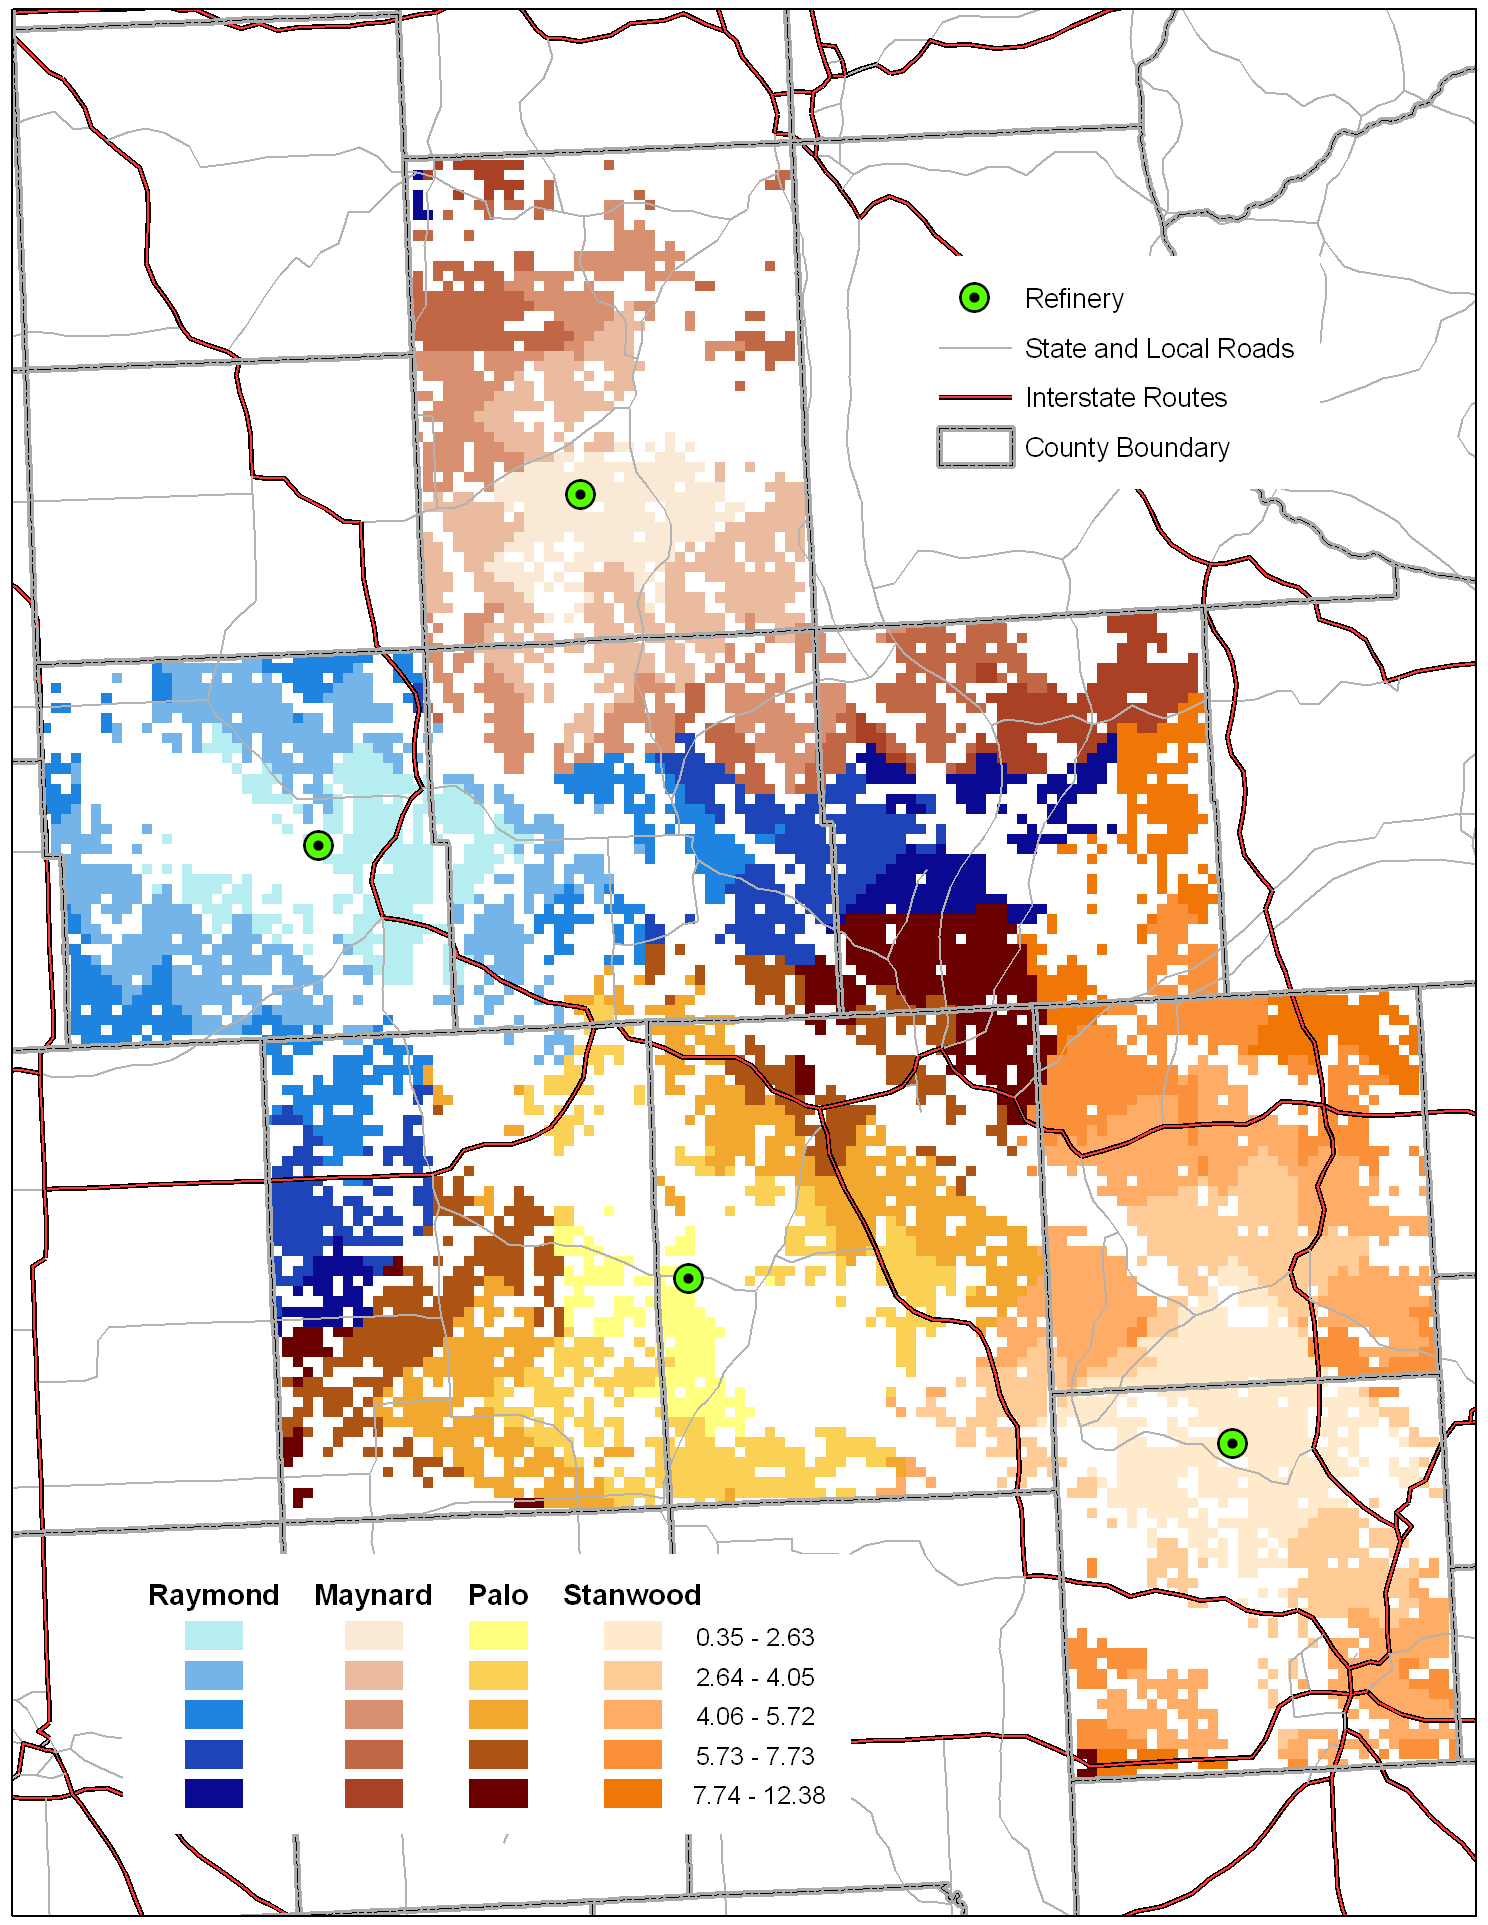
\includegraphics[width=0.45\textwidth]{iowa/farm_costs_travel.png}  
    }
    \caption{Refinery locations and travel costs}
    \label{fig:dest-travel}
\end{figure}


\subsection{Supply curves}

Figure~\ref{fig:supply_curves} shows the individual supply curves for
the 5 refineries in the study region.  The figure shows that despite
the differences in the harvest yields, and transportation
infrastructure, the general shape of the curves are fairly
consistent.

\begin{figure}[hpt]
  \centering
  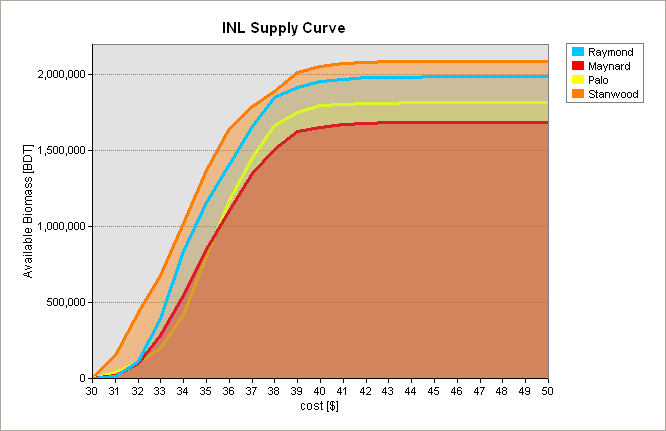
\includegraphics[width=1.0\textwidth]{inlsupplycurve2.png}  
  \caption{Example refinery supply curves for Iowa. }
  \label{fig:supply_curves}
\end{figure}

Figure~\ref{fig:supply_curves_hist} shows this same data as a
histogram, which identifies the range of costs for feedstocks.
Farmgate costs can be affected both by the amount of arable land in
the region as well as by the harvest yields of the biomass.  In
general, however, these vary less than the transportation costs.
Transportation costs are affected by how far the biomass needs to
travel, and in some extent to the speed of the roads being used.
Figures~\ref{fig:farmgate_hist} and~\ref{fig:transportation_hist} show
the various contributions from the farmgate costs and the
transportation costs of the feedstocks

\begin{figure}[hpt]
  \centering
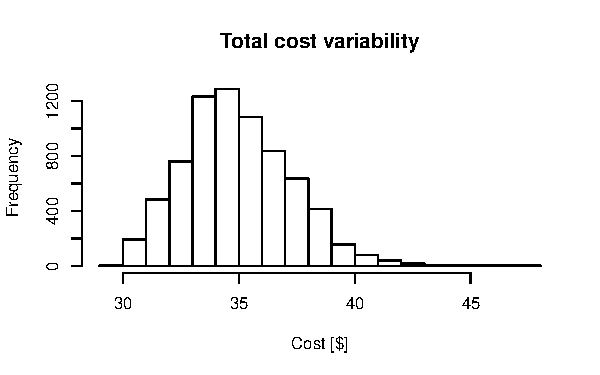
\includegraphics[width=1.0\textwidth]{total.pdf}
  \caption{Total costs \unitfrac{\$}{bdt} of biomass }
  \label{fig:supply_curves_hist}
\end{figure}

\begin{figure}[hpt]
  \centering
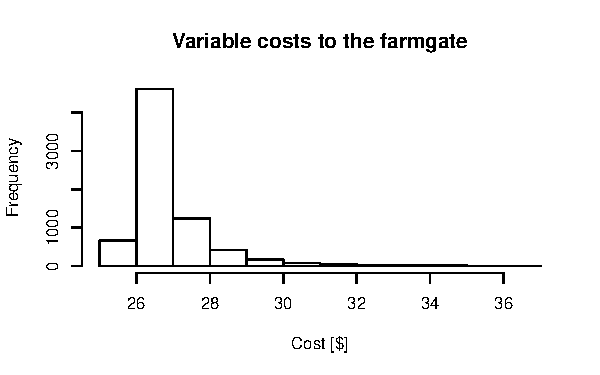
\includegraphics[width=1.0\textwidth]{farmgate.pdf}
  \caption{Farmgate costs \unitfrac{\$}{bdt} }
  \label{fig:farmgate_hist}
\end{figure}

\begin{figure}[hpt]
  \centering
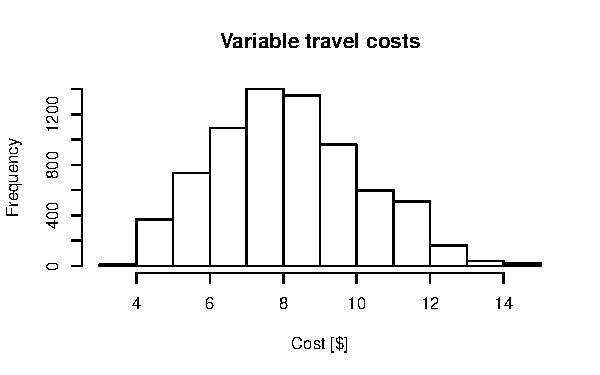
\includegraphics[width=1.0\textwidth]{road_hist.pdf}
  \caption{Transportation costs \unitfrac{\$}{bdt} }
  \label{fig:transportation_hist}
\end{figure}

That transportation is the most variable cost can also be seen in the
utilized feedstock at any given price.  Figure~\ref{fig:supply_curves}
shows that about \%50 of the feedstock is available at \$35.
Figure~\ref{fig:util35} shows the farms that are utilized at this
price.

\begin{figure}[hpt]
  \centering
  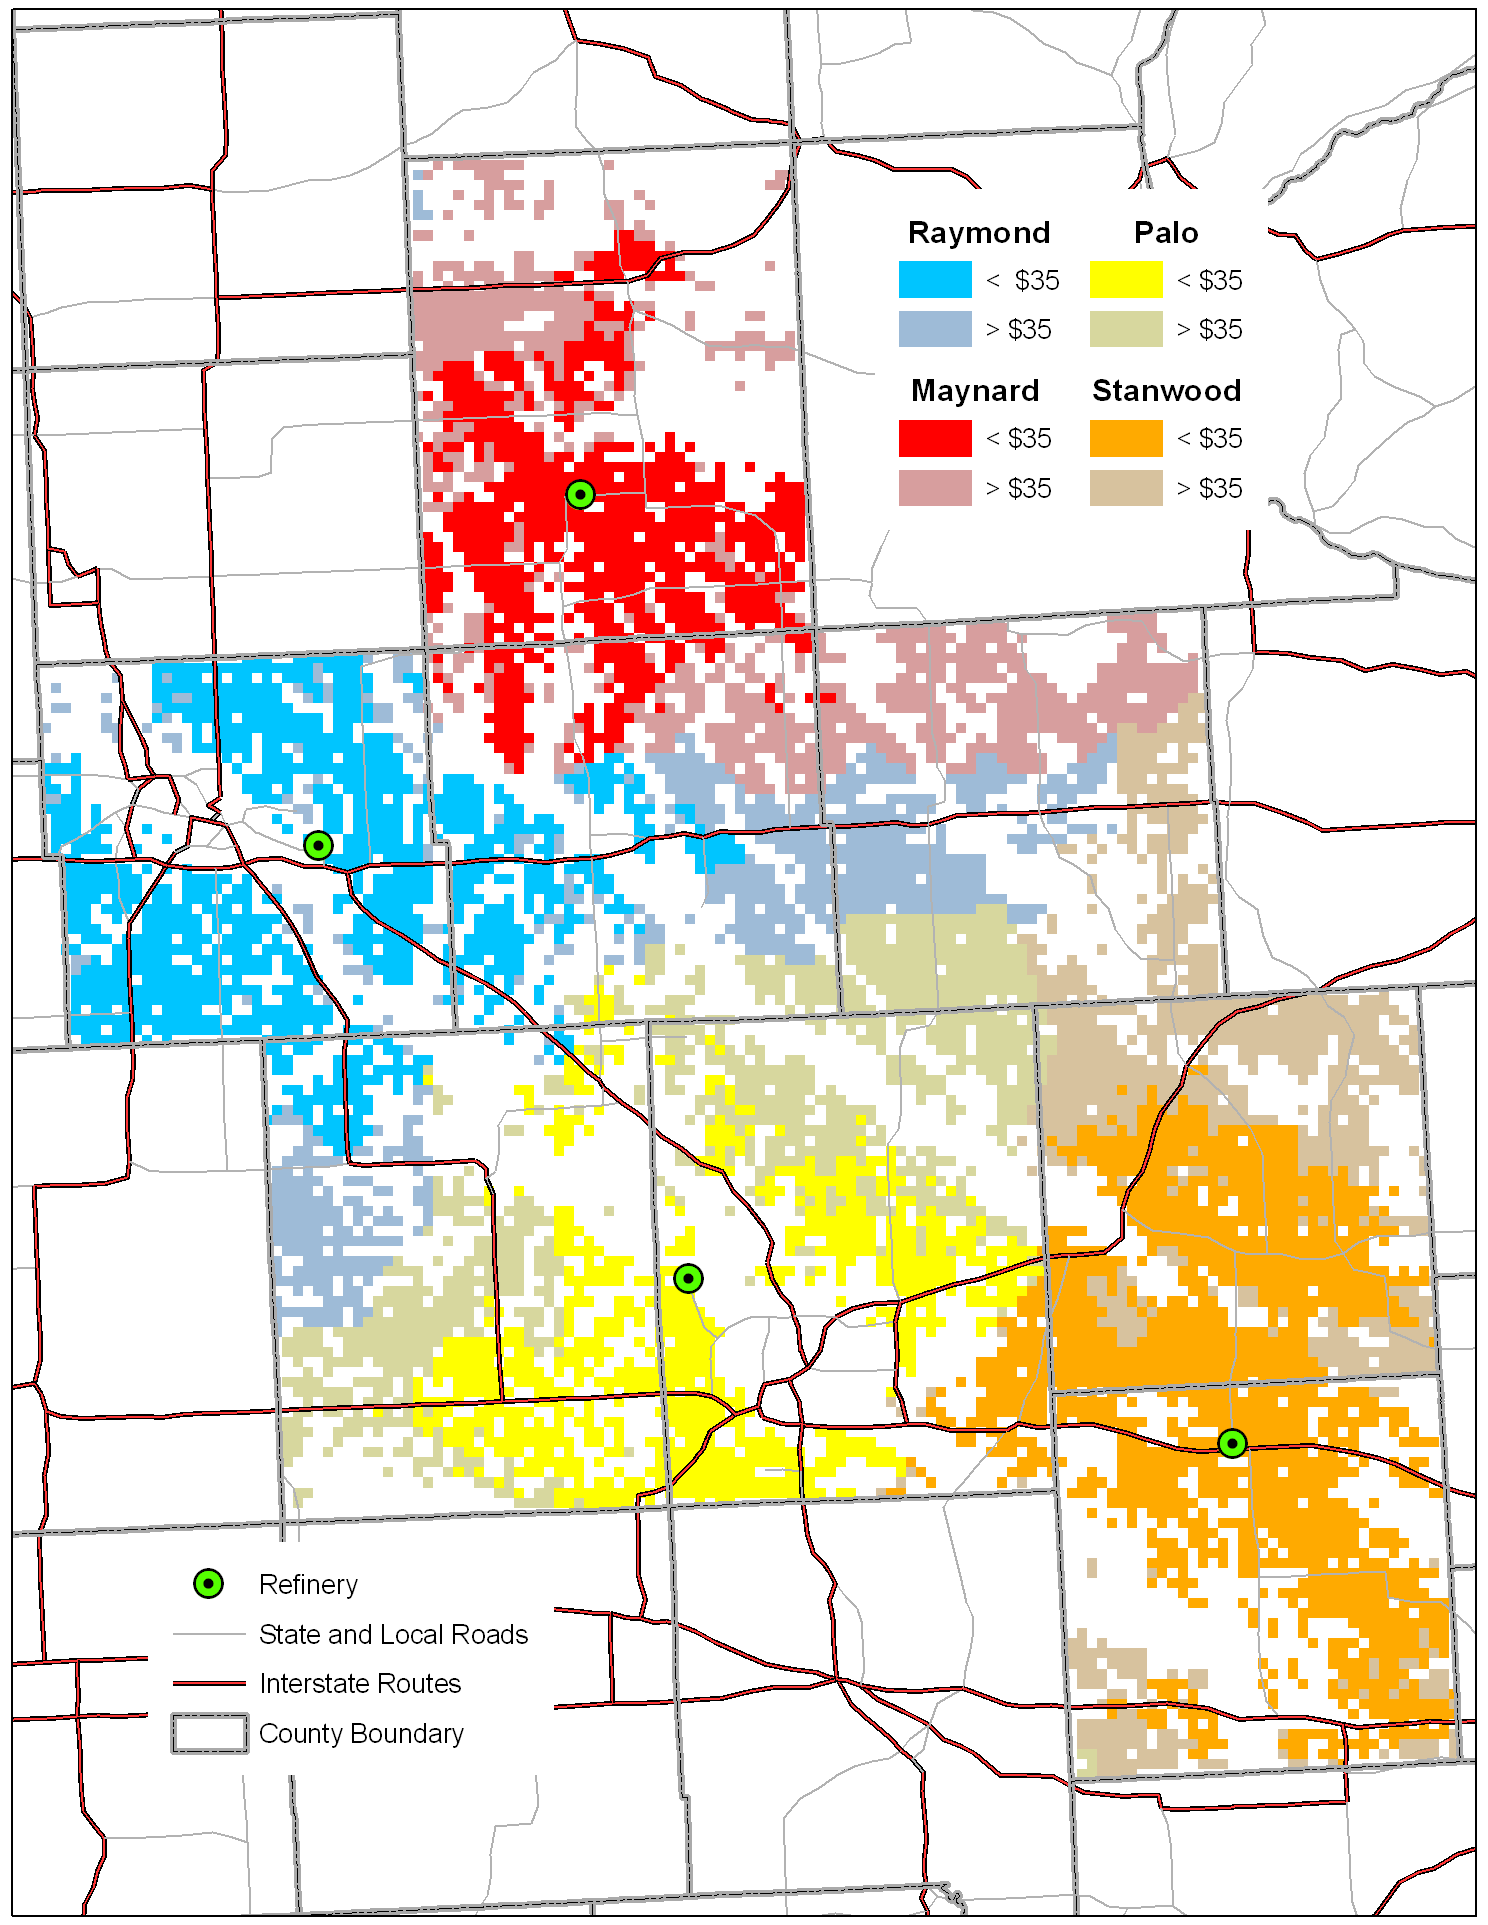
\includegraphics[width=1.0\textwidth]{farm_costs_35dollar_divide.png}  
  \caption{Utilized biomass at \unitfrac[35]{\$}{bdt}. }
  \label{fig:util35}
\end{figure}





\nocite{*}
%\bibliographystyle{elsart-harv}
\bibliographystyle{elsart-num}
\bibliography{wga}

%\appendix{Database Schema}

% \begin{figure*}[htbp]
%   \centering
% %  \epsfig{figure=db/WGA.eps,height=1.0\textwidth,angle=-90}
%   \caption{WGA processing schema}
% \label{fig:process}
% \end{figure*}


%\appendix{Postgres Functions}


\end{document}


% LocalWords:  feedstocks biofuel feedstock farmgate
